\documentclass[journal,onecolumn]{IEEEtran}

\usepackage{cite}

% *** GRAPHICS RELATED PACKAGES ***
%
\ifCLASSINFOpdf
  \usepackage[pdftex]{graphicx}
  \graphicspath{{img/}}
\else
  \usepackage[dvips]{graphicx}
  \graphicspath{{img/}}
\fi

% *** SPECIALIZED LIST PACKAGES ***
%
\usepackage{algorithmic}

\usepackage{array}

% *** PDF, URL AND HYPERLINK PACKAGES ***
%
\usepackage{url}

% correct bad hyphenation here
\hyphenation{op-tical net-works}

\begin{document}

\title{Volunteers in the Clouds: an Architecture for Low Cost and
  Potentially Massive Distributed Evolutionary Computation}

\author{Juan-J.~Merelo*$^1$, Mario Garc\'ia-Valdez$^2$, Pedro A. Castillo$^1$, Pablo Garc\'ia-S\'anchez$^1$
\thanks{Manuscript submitted for review on \today.}%
\thanks{$^1$Dept. of Computer Architecture and Technology and CITIC University of Granada}%
\thanks{$^2$Dept. of Graduate Studies at Instituto Tecnol\'ogico de Tijuana}%
\thanks{E-mail addresses: {\tt jmerelo@ugr.es}, {\tt
    mario@tectijuana.edu.mx}, {\tt pacv@ugr.es}, {\tt pablogarcia@ugr.es}}%
\thanks{*Corresponding author.}%
}

\maketitle

\begin{abstract}
Volunteer computing is used routinely in science and industry, but it
still has a long way to go if it is going to become a mainstream technology in the
same way the cloud technologies in general have. The lack of general
purpose and open source tools
with analytics built in could be one of the reasons why this is so, as
well as the lack of proofs of concept. That is why in this paper we
present {\sf NodIO}, a client-server architecture for distributed
evolutionary algorithms, written entirely in JavaScript, which needs
minimal server support to work and is able to support persistent,
asynchronous, distributed evolutionary algorithms running in the
browser. The architecture, along with some initial results on the
expected performance and scaling
behavior is presented. We also use the algorithm data to
find out what kind of patterns the user behavior follow and try to fit
them to some statistical distribution.
\end{abstract}

\begin{IEEEkeywords}
Evolutionary algorithms, evolutionary computation, distributed computing, internet computing,
social networks, volunteer computing, metacomputing, performance evaluation.
\end{IEEEkeywords}

%---------------------------------------------------------------
\section{Introduction}

\IEEEPARstart{N}{owadays} there is a big and increasing number of
distributed evolutionary computation software frameworks available on
the market, usually as open source systems \cite{Parejo12Survey}. Most of these systems have %FERGU: añadida referencia
two features: they are {\em desktop} applications, that is, they must
be compiled or run directly on the operating system layer and, second,
they assume that the nodes that are going to run the system are under
your control or at least you have access to them.

There is, then, space for systems that do not have any of these
assumptions, such as the one presented in this paper, which will be
provisionally named {\sf NodIO}. {\sf NodIO} is first an application that
runs in two tiers, a server and a client, the latter  can be possibly
run on a  % [Pedro] Both the server and the client in browsers?
          % different browsers as I understand? [JJ]  No, server in
          % server, client in browser, although there's nothing that
          % can't be done in a browser.
browser. As such, it can be run in any computer that loads the web
page where the client is embedded, including many over which%[Mario]Quitar el possibly?   [JJ] Done
the scientist has no control.

Some time ago, our group faced the problem of diminishing funds for
buying new     % [Pedro] This sentence is so so long. I would split it
               % in two sentences. [JJ] Done.
hardware. This was aggravated by the increasing maintenance costs and
extended downtime resulting from the continuous failures of existing
clusters.
Considering this, we leveraged our experience in the design of web
applications, including JavaScript, since their inception and other
volunteer and
unconventional distributed evolutionary computing systems, and we
decided to design and release a new free framework that would allow anyone to
create a volunteer distributed EC experiment using cloud resources as
servers and browsers as clients.

This kind of systems must solve a series of issues before even starting to %FERGU: cambiado el "these systems" porque parecía que hacía referencia a "los anteriores"
measure their performance; these issues are related to security as well as
safety, which introduces a {\em social} aspect to the design of a
computing system that makes it a {\em techno-social system}
\cite{vespignani2009predicting}. In this paper our intention is to
present the {\sf NodIO} framework and analyze it from two different
angles: the purely technical angle, including the decisions that went
into its features, and the social angle, to account on how the persons
that voluntarily choose to enter the web page that runs the system
determine its performance and how it can be modeled and, eventually,
predicted.

The rest of the paper is organized as follows: Next we present the
state of the art (Section \ref{sec:soa}) in web-based distributed
computation systems along with attempts to predict and model its behavior. %FERGU: El IEEE es americano
Then, a detailed description of the proposed system is presented
in Section \ref{sec:description}, followed by the experiments and
obtained results in Section \ref{sec:experiments}.
Finally, conclusions and future lines of work are presented in Section
\ref{sec:conclusion}. 

%---------------------------------------------------------------
\section{State of the art}
\label{sec:soa}

The web used as a resource for distributed computing has a
long history, and almost since the beginning it was used for
evolutionary computation even before JavaScript was
introduced as a browser-based scripting language in 1997. Before that
time other technologies,
 including Flash animations and VBScript, ActiveX or Java applets were
used; for instance, Java was pointed out in \cite{soares1998get} as a
``language for the
internet'', providing some advantages such as multi-architecture compatibility or
security mechanisms and was proposed in \cite{chandy1996world} as the
basis for the creation of a world-wide peer to peer system using Java
compiled programs. The ATLAS system
\cite{Baldeschwieler:1996:TIG:504450.504482} also used Java together
with another language called Cilk; all these papers indicated that
the introduction of an architecture-independent system such as the
Java virtual machine opened the doors for ultrascale, Internet-wide,
metacomputers. This paper also establishes the desirable features of
any {\em global computing} infrastructure, that can also be applied to
distributed evolutionary computation experiments that rely on
volunteer computing: scalability, heterogeneity, fault tolerance,
adaptive parallelism, safety, anonymity, hierarchy, ease of use and
reasonable performance. Of all these, probably {\em hierarchy}, that
is, the capability of using preferentially resources in the same
organization could be either disregarded or included in adaptivity,
leaving us with eight desirable properties.

The fulfillment of these properties could be achieved using any of the
languages and associated technologies, mentioned above, provided that the user had
installed the required virtual machine plugin first, but embedding a
ditributed computation client in the browser has the advantage of
providing a single and universal way of accessing resources via an
URI, something that is not guaranteed using desktop
applications. Baratloo et al. tried in 1996 to create a system with
the aforementioned qualities called {\em Charlotte}
\cite{baratloo1996charlotte}. This system, which implemented a
distributed shared memory, was inspired by previous work
on parallel computing systems PVM and MPI and solved most issues by
using the Java virtual machine embedded in the browser,
which provides
security to the user, uniformity of computing environment
independently of the operating system and access to a common data store in the
server. Since the virtual machine is a sandbox, it is safe to the user
and running a compiled bytecode guarantees a certain level of
performance.
 Other issues such as scheduling, which are related to adaptive
 parallelism, are solved on the server. This
paper was later extended and published in a journal in 1999
\cite{baratloo1999charlotte}, but it is interesting to note that
already in the early stages of the web the possibility of
browser-based distributed computing was already researched.

Other systems, like JET, proposed by Soares et
al. \cite{soares1998get}, also used Java. JET supports
the execution of parallel applications over the Internet and features
a comprehensive statistics collection subsystem, allowing its use for science,
since it allows the collection of algorithm analytics by the
experiment designer, unlike the other systems mentioned
above. Other proposals contemporary to Jet, such as {\em SuperWeb}
\cite{alexandrov1997superweb} are roughly a translation of classical
distribution techniques, with complicated architectures that include
brokers for resource discovery. It is focused, however, in solving the
issues involved in browser-based computing and also in making a system
that is able to work across different classes of computers, mentioning
SPARCstations and PCs with Windows-95. Interestingly enough, this
paper incorporates a discussion on the economic model, paving the way
for the for-profit distributed computing systems that later on
arose. On the other hand, the potential for volunteer computing using
browsers was realized
later on \cite{sarmenta-bayanihan} as well as the potential for
mischief of users with code in their hands
\cite{sarmenta-sabotagetolerance}. However, these early efforts by
Sarmenta once again used Java and not JavaScript, making this effort
less widespread.

The main problem with Java and all the other browser-embedded
technologies is that they are not {\em universal} in the
sense than an extra component, namely, the Java virtual machine or another
virtual environment has to be installed in the browser.
Also these virtual environments have become targets of malicious attacks; 
for instance numerous vulnerabilities have been discovered in 
the proprietary Adobe Flash runtime environment and
video player \cite{ford2009analyzing,watanabe2010new}. The need for
these additional environments has been mitigated with the
adoption of the HTML5 standard \cite{anthes2012html5}.
JavaScript, however,
\cite{flanagan2006javascript} was introduced in 1997 as a
browser-embedded language and has, since then, become a set of standards
\cite{ECMA-262} that include the language and its components. Since
early on, it was adopted by the industry and also by scientists,
who used them for creating an EA on
the browser as early as 1998 \cite{jj-ppsn98}.

JavaScript can be used either for unwitting
\cite{unwitting-ec} or volunteer
\cite{langdon:2005:metas,gecco07:workshop:dcor} distributed
evolutionary computation and it has been used ever since by several
authors, including more recent efforts
\cite{Desell:2008:AHG:1389095.1389273,duda2013distributed,DBLP:journals/corr/abs-0801-1210} 
that even
used the client's GPU \cite{duda2013gpu} or create an object-oriented
framework for evolution in the browser \cite{EvoStar2014:jsEO}. Many other researchers have
used Java \cite{chong:1999:jDGPi} and others have gone away from the
server-based paradigm to embrace peer to peer systems
\cite{jin2006constructing,10.1109/ICICSE.2008.99,DBLP:conf/3pgcic/GuervosMFEL12}. These computing
platforms avoid single points of failure (the server) but, since they
need a certain amount of infrastructure installed to start, the
threshold to join them is much lower.

Recent works propose the use of cloud computing services for the components of
client-server distributed EAs. Cloud resources
can reduce operational costs by outsourcing both hardware and software maintenance
to the cloud provider. Another advantage is that they enable the provisioning of computing resources beyond what
is available in most laboratories, allowing researches to
scale algorithms at reasonable costs. Researchers have proposed the use of
public clouds such as Amazon EC2 \cite{CloudScale}, Google App Engine\cite{di2013towards}
and DropBox~\cite{mericloud}. The use of JavaScript to implement
server side components
gives software developers certain advantages in the cloud
paradigm, since is a first-classe citizen
in most Platforms as a Service (PaaS) products as most support the {\tt node.js}
framework \cite{wood13:nodejs:paas}. Many web services
have native JavaScript libraries too, and use JSON (JavaScript Object Notation) for data
interchange. Another advantage is that
developers can use the same software tools for both client and server
side development.

JavaScript is also compatible with the functional programming paradigm \cite{Cousineau1998,MacLennan1990,Thompson1996}.
According to \cite{swanresearch2015}, the benefits of using this kind of paradigm in
metaheuristics optimization allows an improvement in communicability,
reproducibility, interoperability, automated assembly, knowledge engineering
and efficiency.

In the work presented in this paper, JavaScript has been used throughout the full
stack, which has the advantage of using the self-same lines of code for
writing an evolutionary algorithm for the
desktop or command line and browser clients, both based in the EC
library NodEO \cite{DBLP:conf/gecco/GuervosVGES14}. This saves time 
when writing code and leverages 
expertise acquired in the library itself. 

On the other hand, we are also interested in measuring the performance
of volunteer computing systems, an area in which there have been
relatively few efforts.
There were some initial attempts to avoid the differences in performance
that could be obtained from volunteers  by making
the algorithm adaptive to the kind of resources allotted to it
\cite{milani2004online}, which is actually not such a big problem in
algorithms such as the EA that can easily be
parallelized via population splitting or farming out evaluations to all
the nodes available. Lately, several approaches have focused on the
fault-tolerance of volunteer algorithms
\cite{gonzalez2010characterizing} which can, of course, be studied in
a more general distributed computing context
\cite{nogueras2015studying} or including it in a more general study of the
performance of the EA itself
\cite{DBLP:journals/gpem/LaredoBGVAGF14}.

On the other hand, measuring performance of the resulting metacomputer
involves understanding the dynamics of this kind of systems. Initial
work was done for peer to peer systems by Stutzbach et
al. \cite{stutzbach2006understanding} and extended to volunteer
computing by Laredo et al. \cite{churn08,laredo2008rcp}. But the raw material of
volunteer computing, number of users and the time spent by every one in the
computation in browser-based volunteer computing experiments, have
only been studied in a limited way in 
\cite{DBLP:journals/gpem/LaredoBGVAGF14} on the basis of a single
run. Studies using volunteer computing platforms such as SETI@home
\cite{javadi2009mining} found out that the Weibull, log-normal and
Gamma distribution 
modeled quite well the availability of resources in several clusters
of that framework; the shape of those distributions is a skewed bell
with more resources in the {\em low} areas than in the high areas:
there are many users that give a small amount of cycles, while there
are just a few that give many cycles. This is in concordance with the
results obtained in \cite{agajaj}. Our initial tests indicate that
this kind of distribution might be the most appropriate to describe
user participation in several different metrics. However, in this
paper we will perform different experiments in different setups and
will try to come up with a more precise model. Next we describe the
system itself.


As far as we know, this paper presents one of the few experiments that
uses computational resources that are as dissimilar as smartphones and
powerful laptops 
or desktop computers in a research center. The methodology used to
gather resources and the algorithms used will be described next, as
well as the results obtained with the setup.

%---------------------------------------------------------------
\section{Description of the system}
\label{sec:description}

In general, a volunteer-based distributed evolutionary computation
system based on the browser is simply a client-server architecture
whose client is, or can be, embedded in the browser via JavaScript.

In this sense, in this paper we propose {\sf NodIO}, a cloud or metal
based 
volunteer evolutionary computing system based on the {\sf NodEO}
library, whose architecture 
has been developed using JavaScript on the client as well as the
server sides. 
All parts of the system are free and available with a free
license from \url{https://github.com/JJ/splash-volunteer}.
Thus, {\sf NodIO} architecture has two tiers:\begin{enumerate}
\item A REST server, that is, a server that includes several {\em
  routes} %remote requests suena raro, propongo algo como: remote
          %procedures o web interfaces [jj] changed to routes, its
          %proper name.
  that can be called for storing and retrieving information (the CRUD cycle:
  create, request, update and delete) from the server. The information
  is of two kinds: {\em problem} based, that is, related to the
  evolutionary algorithm such as {\tt PUT}ing a chromosome in or {\tt
    GET}ing a random chromosome from it, and {\em information} related
  to performance and state of the experiments. It also performs logging
  duties, but is basically a very lightweight and high performance
  data store \cite{jj:idc:lowcost}.
  The server has the capability to
  run a single experiment, storing the chromosomes in a data structure
  that is reset when the solution is found.
\item A client that includes the evolutionary algorithm as
  JavaScript code embedded in a web page that displays graphs and some
  additional links and information on the experiment. This code runs
  an evolutionary algorithm {\em island} starting with random
  population and sending, every 100 generations, the best individual
  back to the server (via a {\tt PUT} request) and requesting a random
  individual from the server (via a {\tt GET} request). Apart from
  these constants, the algorithm can be run in many different ways:
  stopping when solution is found or, as we have done in this paper,
  using WebWorkers, which run in the background even if the webpage or
  browser tab with the experiment is not currently on focus.
\end{enumerate}

Figure \ref{fig:system} describes the general system architecture and
algorithm behavior. Different web technologies, such as JQuery or {\tt
  chart.js} have
been used to build the elements of the system.
\begin{figure}[!t]
\centering
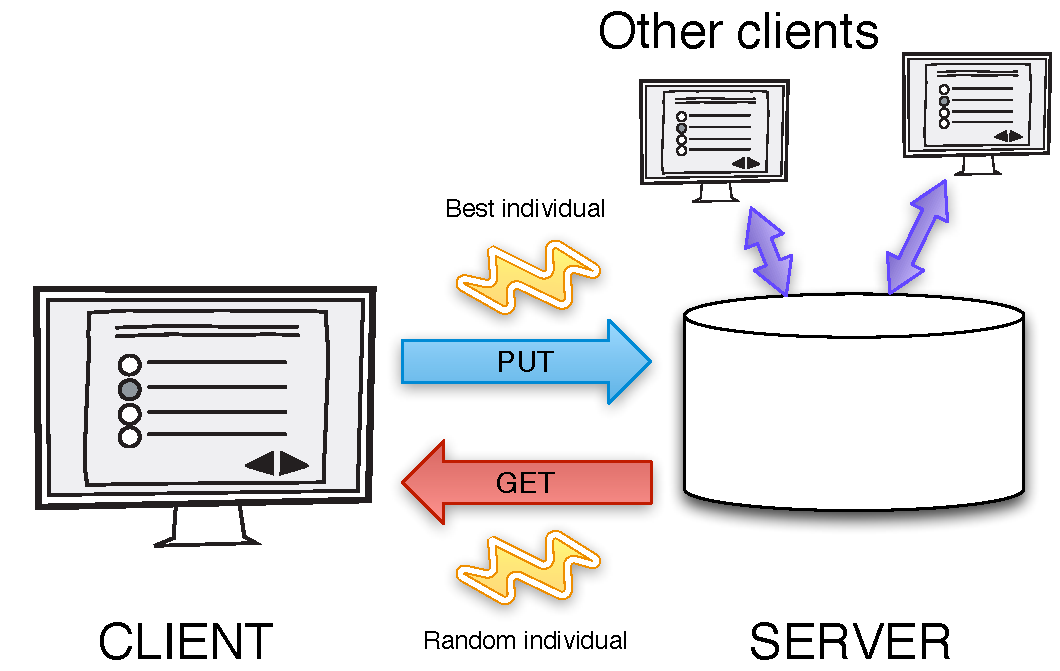
\includegraphics[width=4in]{img/system.pdf}
\caption{Description of the proposed system. Clients execute a JS EA
  in the browser, which, every 100 generations, sends the best
  individual and receives a random one from the server. }
\label{fig:system}
\end{figure}

The researcher only has to change a function to solve a different
problem, in this case the classical Trap function \cite{Ackley1987} has been
used. JavaScript is a functional language and declaring a different
function and handing at the creation of the algorithm object, called
{\tt Classic} is the only change needed to work with a different
problem. Let us see how this system addresses the different challenges
outlined in the State of the Art (Section \ref{sec:soa}):\begin{itemize}
\item {\em Scalability} is provided via the use of a lightweight and
  high-performance, single-threaded, server based in NodeJS and
  Express.js. Although this single server is a bottleneck since it
  will eventually saturate, the fact that it runs as a single thread
  allows the service of many requests. In fact, a limit with the
  number of simultaneous requests will be reached, but so far it has
  not been found, unlike what we found in our previous systems, DCoR,
  \cite{gecco07:workshop:dcor}, which had a low scalability.
\item The system is {\em heterogeneous} since it does not need any
  performance, operating system or even browser requirement: anyone
  visiting the page, even from mobile devices, can load the algorithm.
\item {\em Fault tolerance} is always an issue, and in this case, the
  single point of failure would be the server: the system, as such,
  would break down if the server fails. However, the individual
  islands in every browser would continue running, and having access
  to just one of them would allow the local algorithm to proceed. In
  fact, the island does not need the server to run: it runs locally if
  needed, with the only exception that it is obviously unable to
  communicate with the rest of the islands.
\item {\em Adaptiveness} is achieved simply through autonomous
  operation of every individual island and no synchronization
  mechanism. The islands in the system are, in fact, unaware of each
  other, communicating only through the server.
\item Since the algorithm is run on the browser, {\em safety} is
  achieved through its sandbox mechanisms. The user is thus assured
  that there is no unsafe access either to their local files or even
  to more resources that the browser should be allotted.
\item Running the algorithm is just a matter of loading the page,
  which means that operation is totally {\em anonymous}. For the same
  reason, {\em ease of use} is optimal, being as easy as simply
  clicking on an URL and available to anyone with access to a browser.
\item {\em Reasonable performance} is not ensured. In fact, we should
  make sure that there is a reasonable amount of clients over which
  the performance achieved is bigger than what you would obtain in
  your own desktop system. If that is not done, it is a pointless
  academic exercise.
\end{itemize}

This last point is what we will try to prove in the next section.

%---------------------------------------------------------------
\section{Experiments and obtained results}
\label{sec:experiments}

\begin{figure}[!t]
\centering
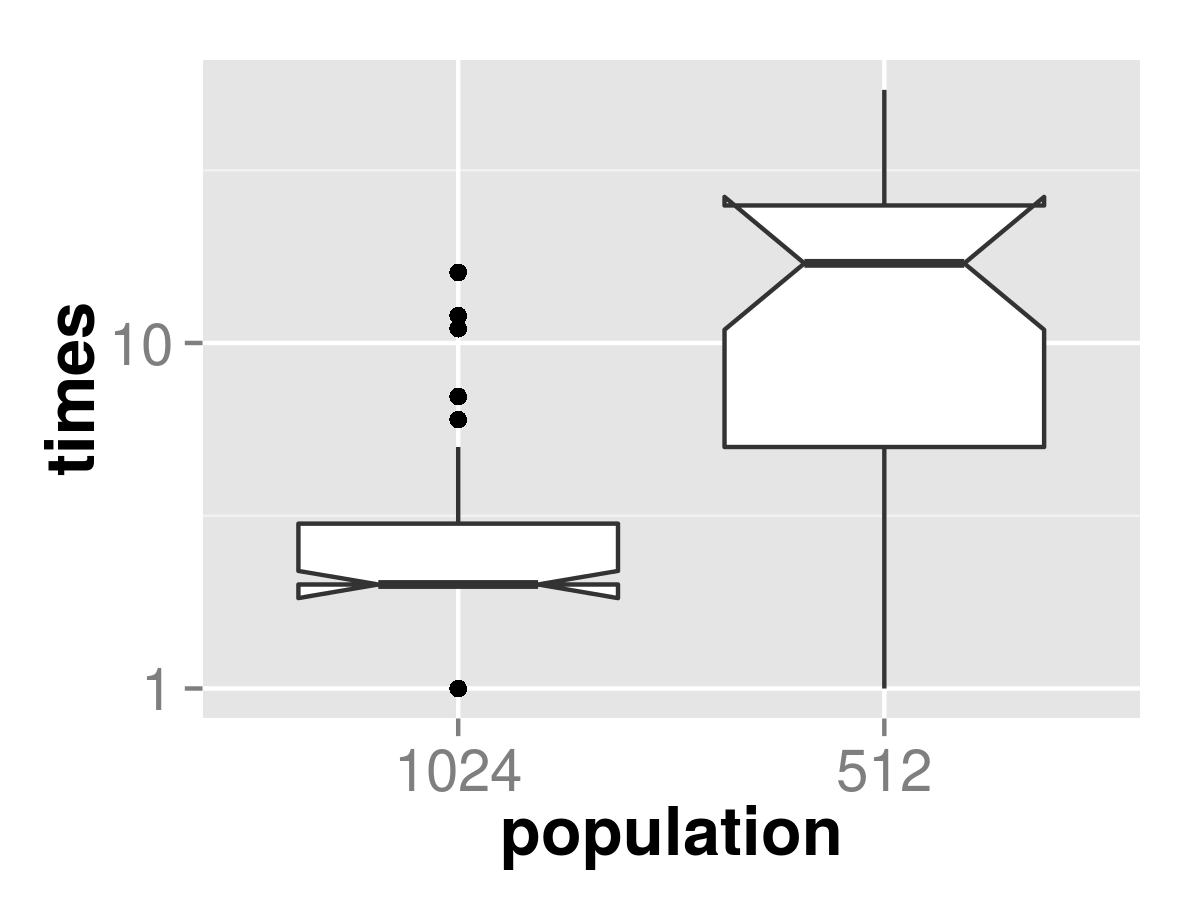
\includegraphics[width=12cm]{img/baseline-times.png}
\caption{Comparison of time to solution for the baseline system, using a {\tt
    node.js} client, for different population sizes. Only
runs in which solution has been found are used for this graph.}
\label{fig:baseline}
\end{figure}
First, we establish the baseline performance by running the
evolutionary algorithm in a desktop client written using NodEO
\cite{nodeo2014}, the basic JavaScript library we have used as base to
build {\sf NodIO}, the framework. This experiment tries to 
find the solution to the 40-trap function with parameters $l=4, a=1,
b=2, z=3$ and a population size equal to 512. The algorithm in a
single island was run until the solution (a string with all
ones) was found or five million evaluations had been performed. It
took around a minute, on average, that is $68.9694$ seconds, to
perform the fifty runs. In this experiment only 33, that is, 66\% were
successful. The experiments were repeated for population $p=1024$,
with success rate upgraded to 100\% and average duration $3.46$
seconds. Results for these two experiments
are shown in Figure \ref{fig:baseline}. %Fergu: dejar claro que es solo una isla

These two experiments establish first a baseline result and show that
time to success depends on the population, with bigger population
contributing more diversity and thus speeding up the solution \cite{DBLP:conf/lion/LaredoDFGB13}. The volunteer computing
experiments that we 
%FERGU: explicar un poco más lo de "depends on the population"?, por ejemplo añadiendo
%as this is a deceptive problem, and low levels or diversity may not help to
%find the solution \cite{} o algo parecido.
%hecho [JJ]
will describe next do not and can not have the same conditions, but
the baseline is that if they eventually take longer than a basic
desktop, their interest will be purely academic. We will try and
prove next that that target performance can be achieved by carrying
out several experiments in different conditions. Second, they also act
as a basic performance test for the server, and also prove that the
basic server can be used for many kinds of different setups, as long
as they follow the REST protocol to deposit and obtain individuals
from the pool. It is obvious that, in this case, the server is not
really needed, since there is a single client and no interaction
between them, but there is a cost in sending and obtaining chromosomes
from the server so it is included for the sake of fairer comparison.

\subsection{Volunteer evolutionary computation: first experiments and results}

Initial experiments were set up using the OpenShift
PaaS, which provides a free tier within which this %Ya se defnió antes PaaS
experiment could be performed. That way, and as required, the hardware
and cloud cost for this experiment were zero. Experiments were
announced through a post in Twitter and other social networks, and
results were published here \cite{DBLP:conf/gecco/GuervosG15}. For the
purpose of this paper, we repeated the announcement several times
through the months of April and then by the beginning of August. All
in all, we have the set of runs with the characteristics shown in
Table \ref{tab:runs}. In general, every experiment took several
days. No particular care was taken about the time of the announcement
or the particular wording. Every {\em experiment} consisted in running
until the solution of the 40-trap problem was found. When the correct
solution was sent to the server, the counter was updated and the pool
of solutions reset to the void set. No special care was taken to wait
until all clients had finished, thus it might happen that, in fact,
the islands running in the browser {\em spill} from one experiment to
the next. However, previous experiments have proven that the influence
of these islands in the next experiment is, in fact negligible.
%
\begin{table*}
\caption{Characteristics of the volunteer computing initial runs. \label{tab:runs}}
\begin{center}
\begin{tabular}{l|rr}
\hline
Date & \# experiments & Different IPs \\
\hline
April 4th 4/4 & 57 & 191 \\
April 24th 4/24 &  231 & 559 \\
July 31th 7/31 & 97 & 179 \\
\hline
\end{tabular}
\end{center}
\end{table*}
%
\begin{table*}
\caption{Summary of time per run, number of IPS and number of {\tt
    PUT}s per IP in the initial runs. \label{tab:summary:os}}
\begin{center}
\begin{tabular}{l|ccccccc}
\hline
Date & Median \#IPs & Max \#IPs & Median time (s) & Median \#{\tt
  PUT}s & $<$ 69s & $<$ 3.46s & Inter-experiment correlation\\
\hline
4/4 & 5 & 16 & 2040 & 18 & 14.29\% & 5.36\% & 0.0082 \\
4/24 &  5 & 29 & 732 & 11 & 47.39\% & 3.91\% & 0.0934\\
7/31 & 5 & 14 & 260 & 23 & 27.08\% & 1.04\%  & 0.1741\\
\hline
\end{tabular}
\end{center}
\end{table*}
%
The table shows that every run included more than 50 experiments. The
%FERGU: No debería ser mejor al revés? Cada experimento está compuesto
%de varias runs. De todas maneras arriba lo has definido así, así que
%si no quieres no lo cambies. Pero me parece más correcto que un
%experimento tenga runs, en vez de al revés [jj] Pues no lo sé. Habría
%que cambiarlo todo. Yo creo que con que sea consisente...
number of different IPs intervening in them varied from more than one
hundred to more than five hundred in the second experiment.

A summary of the results of each run is also shown in Table
\ref{tab:summary:os}. This table shows the median number of IPs
intervening in each experiment,  median of the time needed
to finish the experiment, median number of HTTP {\tt PUT}s per IP, and
then two columns showing the percentage of experiments that took less
than the two baseline experiments shown in the introduction to this
section. The first striking result is that in all cases, 50\% of the
experiments involved 5 or less IPs. This is consistent with results
found previously \cite{DBLP:conf/gecco/GuervosG15} which found 6 to be
the usual number of IPs that participated in an experiment. The
maximum number of different IPs for each experiment is also in the
same ballpark and of the order of 10, which is also consistent with
prior work. The median time has a big range of variation, but 50\% of
the time takes less than several minutes, from around 4 minutes in the
best case to roughly 2/3 of an hour in the worst case. That figure is
not competitive, {\em a priori}, with the baseline experiment, that is
why it is interesting to look at the last two columns, that measure
the percentage of experiments in which the solution was found in less
time than the baseline. It is similar in all three cases, with around
20\% on average for the first baseline experiment, roughly 3\% in the
second case. The comparison is not totally fair: this experiment takes
place in a browser, and in fact most of the time is devoted to
presenting the charts; the server is not the same since it is run in a
PaaS instead of a high-performance desktop computer, and it is also a
remote server, not a local server as in the baseline experiment. But
fair is fair, and we were looking for creating a framework that
allowed to run evolutionary computation experiments {\em faster} than
in our very own computer. And the results is that although it will
happen, 1 out of roughly 5 or roughly 20, depending on what baseline
%FERGU: one->1? OK [JJ]
experiment you choose, it will not happen always or even a majority of
the time. One of the problems is shown in the last column, which
indicates the statistical correlation between the number of IPs
participating in one experiment and the next. In all cases,
correlation is so low as to affirm that there is almost no
relationship between them, that is, computing nodes are not {\em
  staying} after the solution has been found; this is a feature of
this implementation: the user has to actively reload the page to make
the evolutionary algorithm start again. However, it puts a probably
unnecessary cap on the time, or number of experiments, that a user
%Fergu: user no tiene "an", me lo dijo paloma. es "yuser", no "iuser",
%por eso no lo tiene :P 
will voluntarily perform.

\begin{figure}[!htb]
\centering
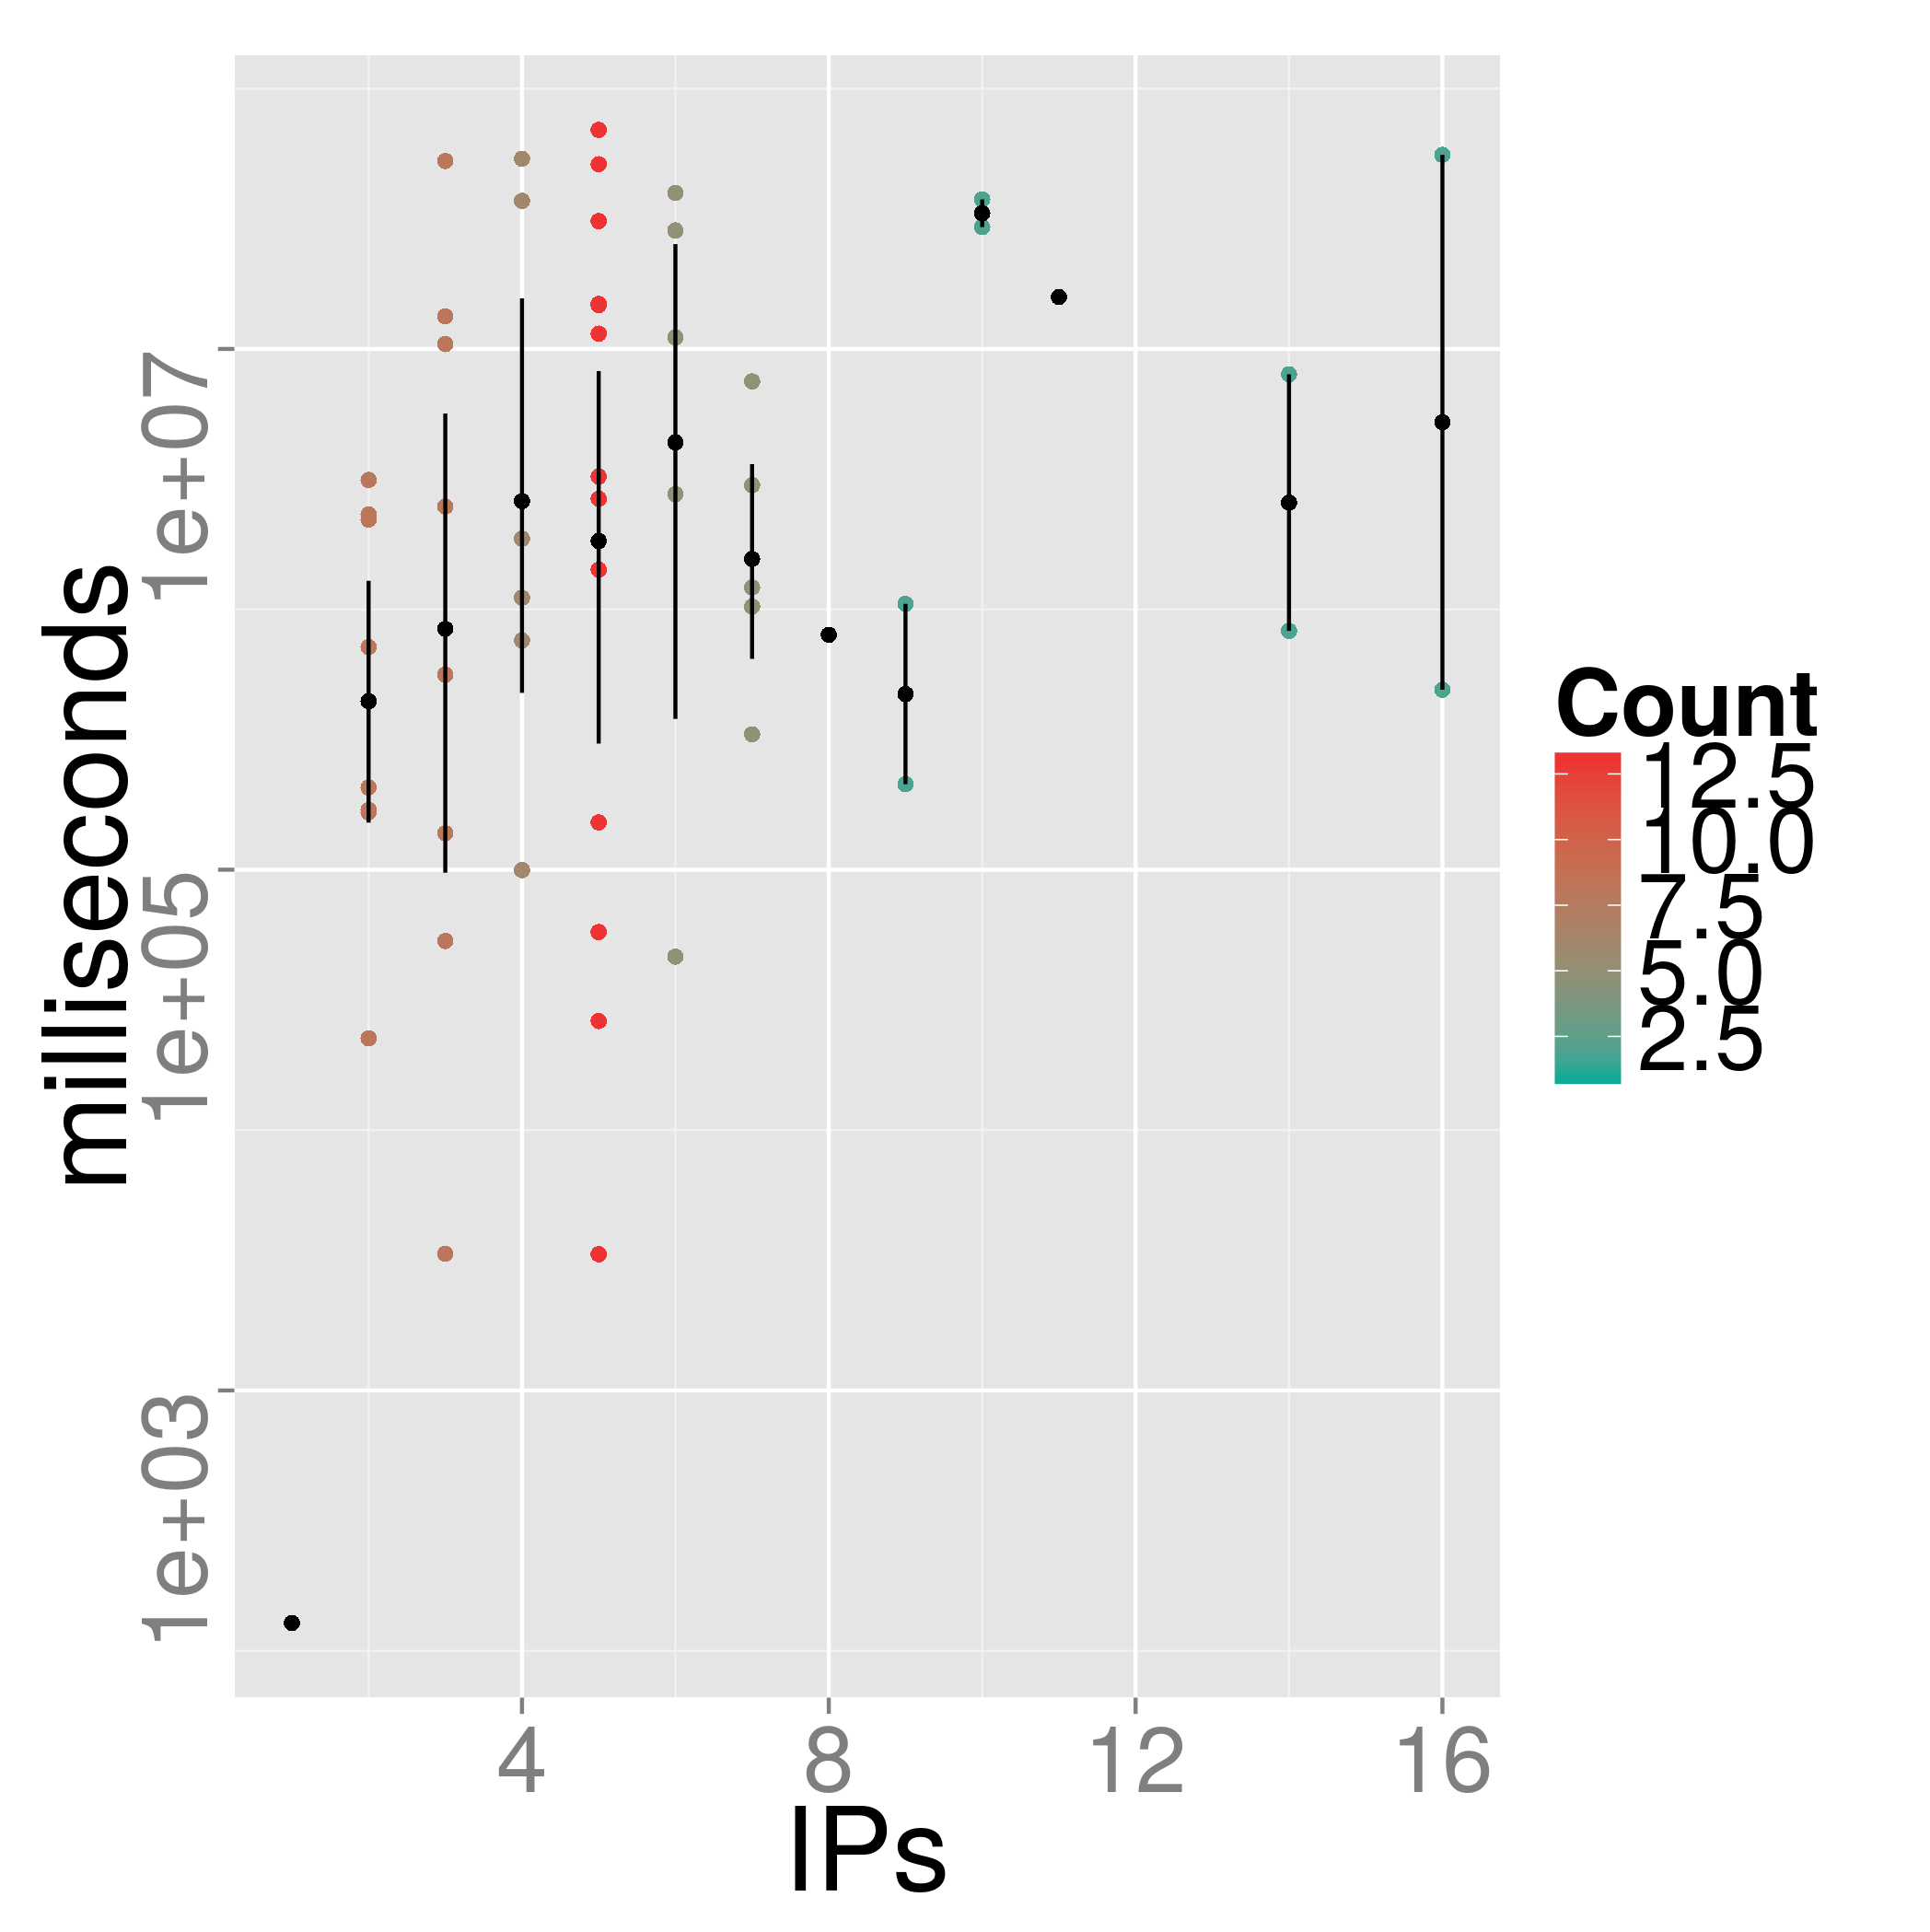
\includegraphics[width=0.32\linewidth]{img/time-vs-ips-OS-4-4.png}
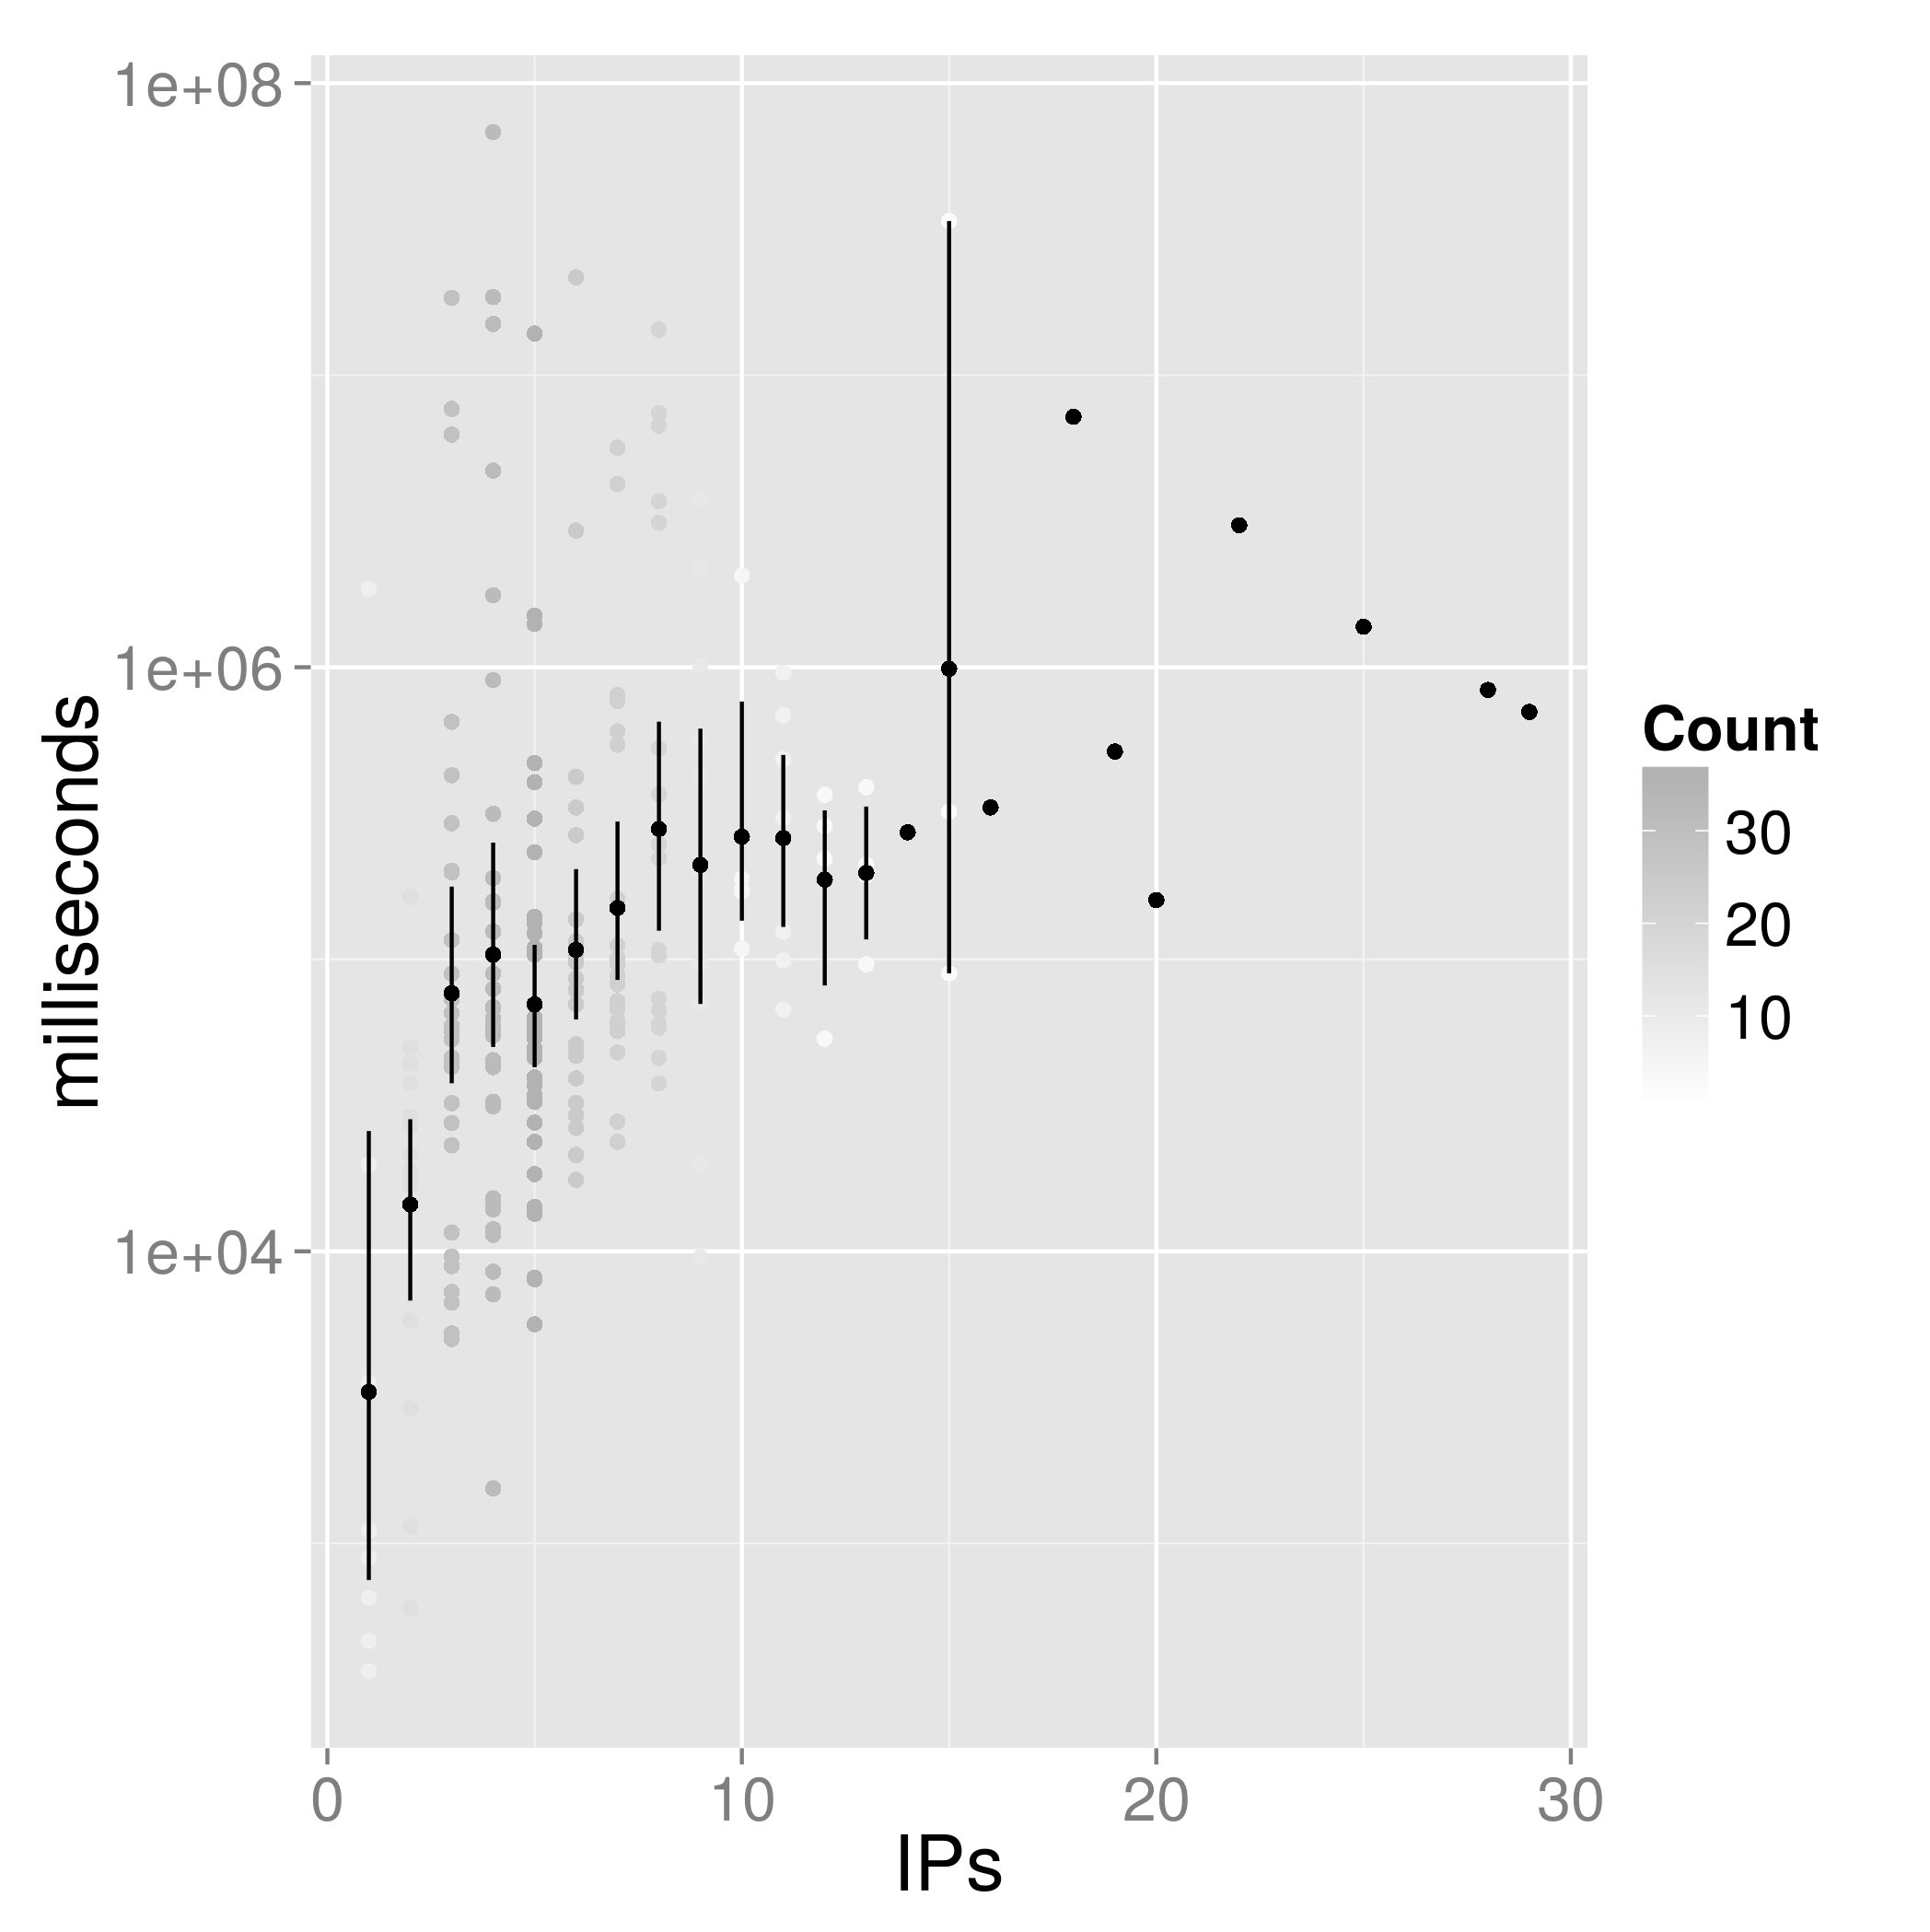
\includegraphics[width=0.32\linewidth]{img/time-vs-ips-OS-4-24.png}
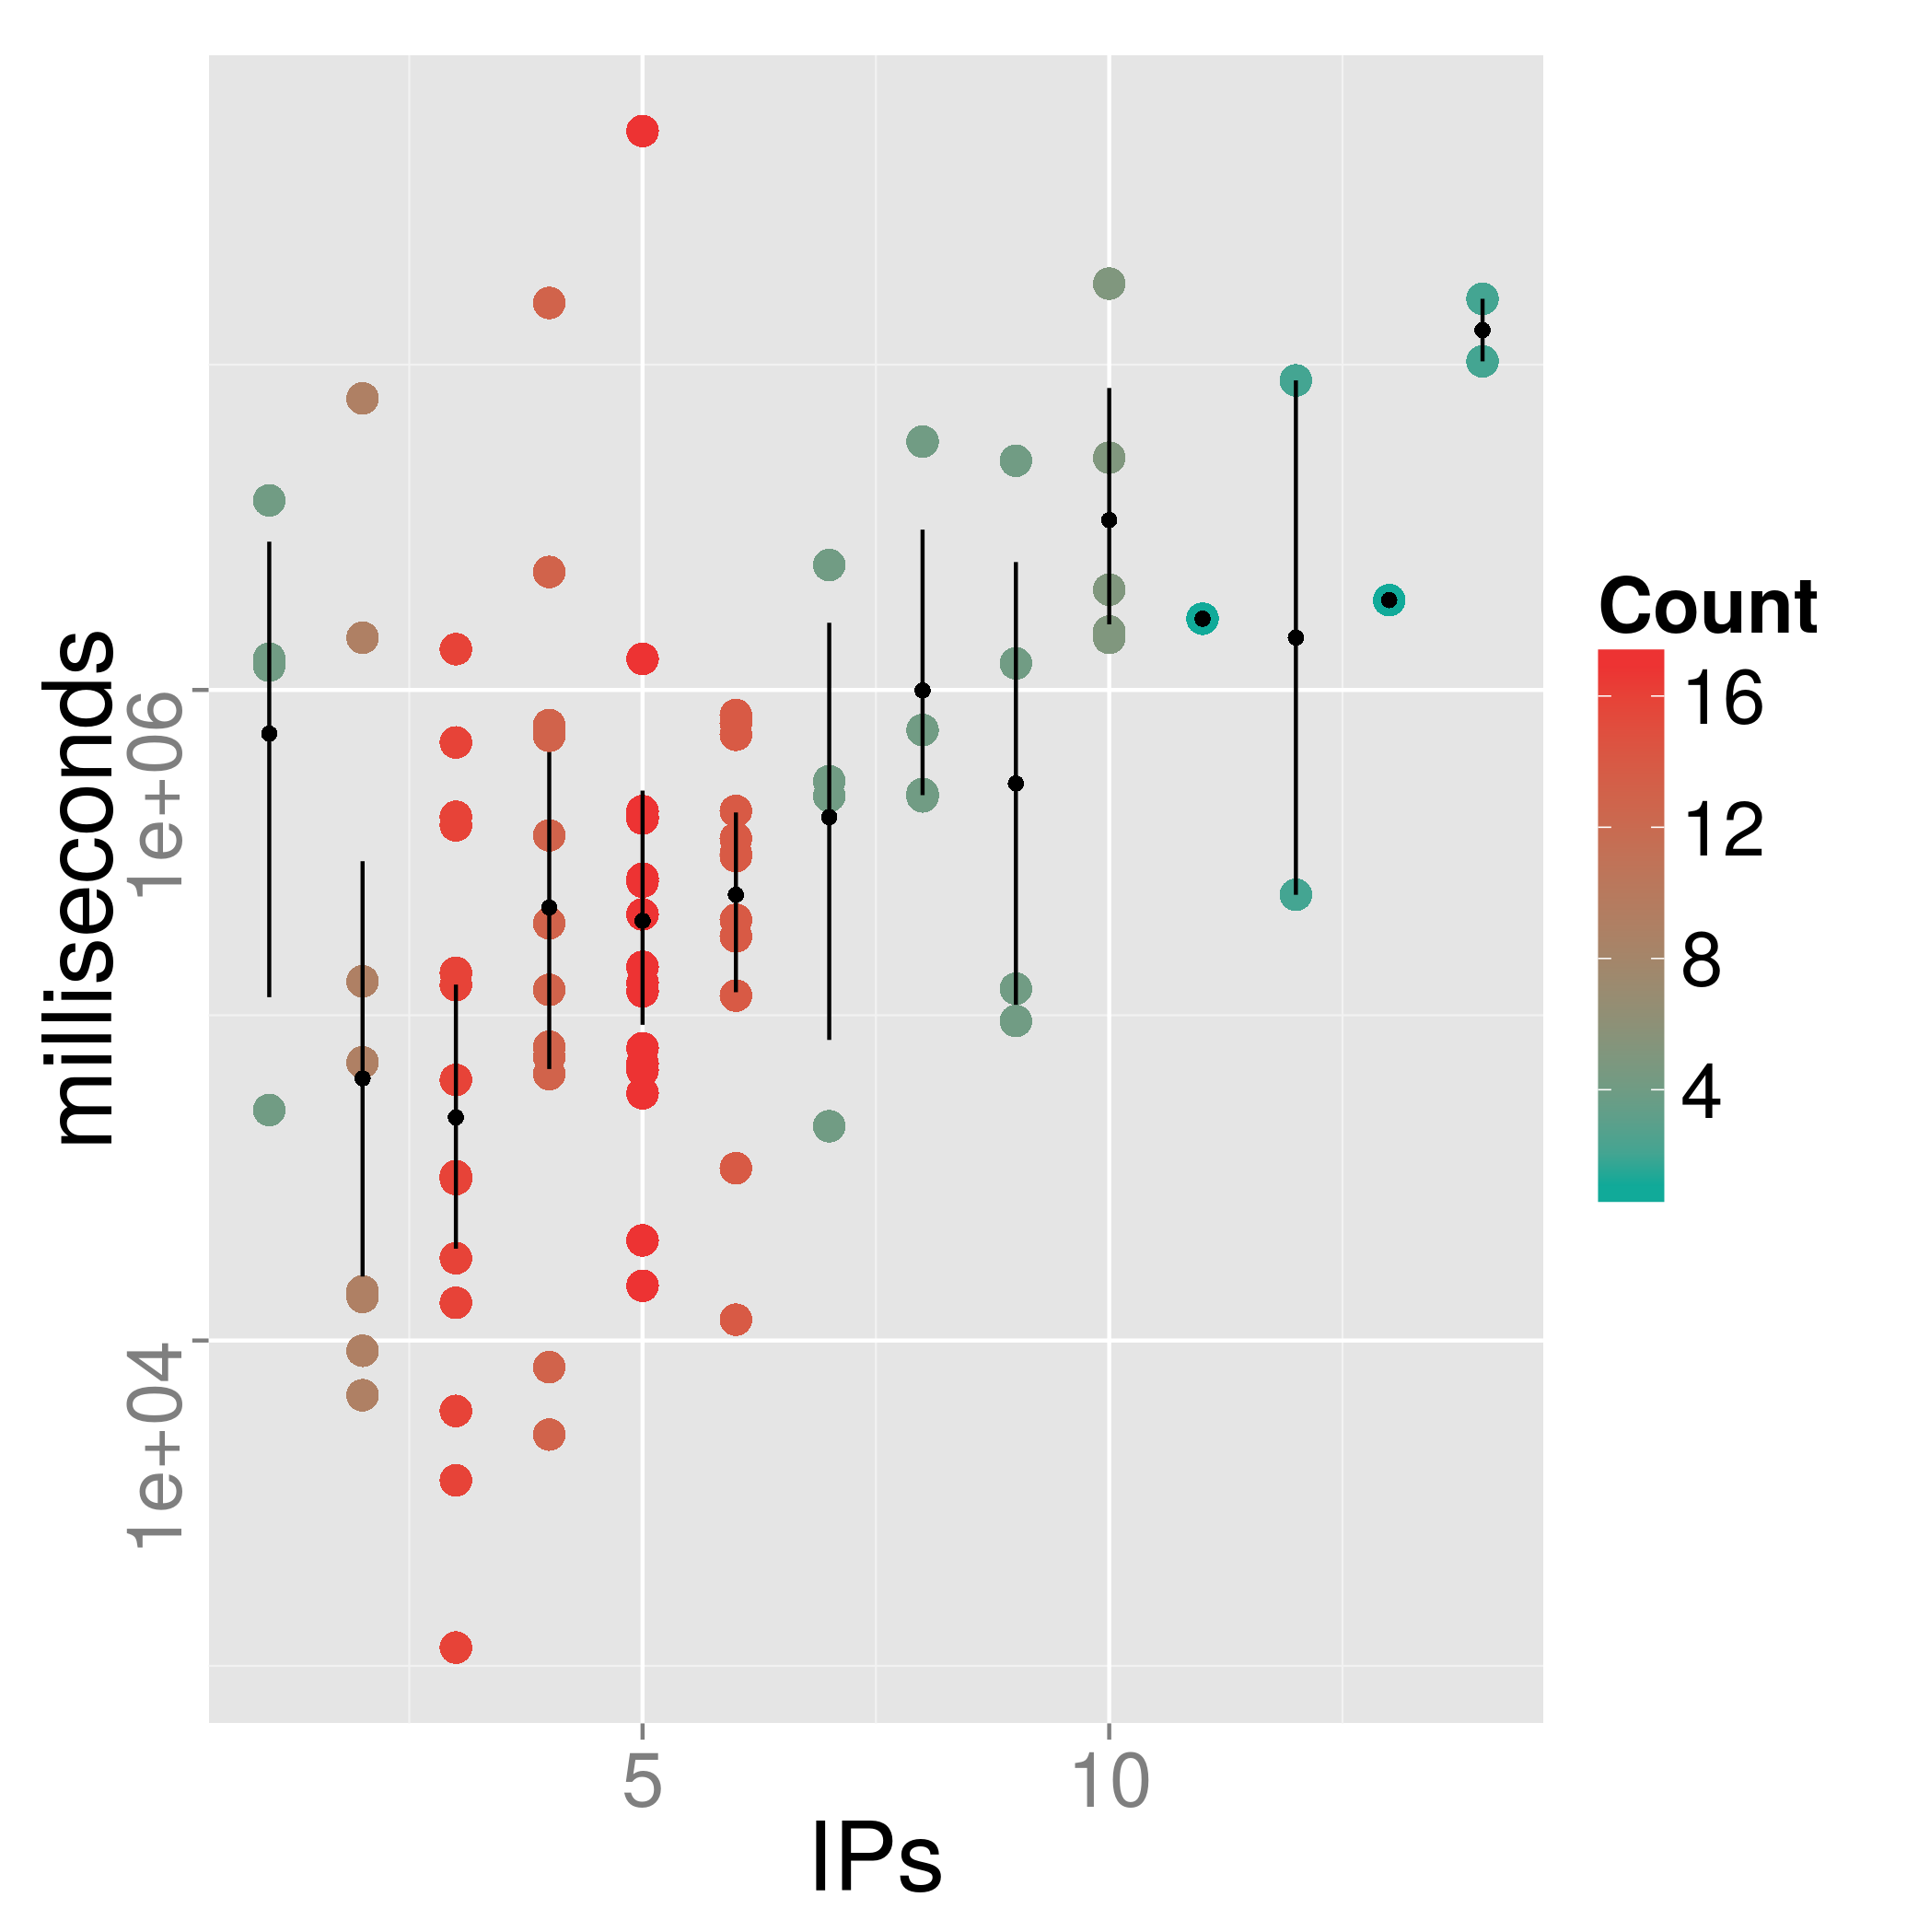
\includegraphics[width=0.32\linewidth]{img/time-vs-ips-OS-7-31.png}
\caption{Duration of experiments vs. number of different IPs (nodes)
  participating in it, with averages and standard deviation shown as
  red dots. From left to right, experiments 4/4, 4/24 and 7/31. Shades
of blue indicate how many experiments included that many unique IPs.}
\label{fig:duration}
\end{figure}
%
\begin{figure}[!htb]
\centering
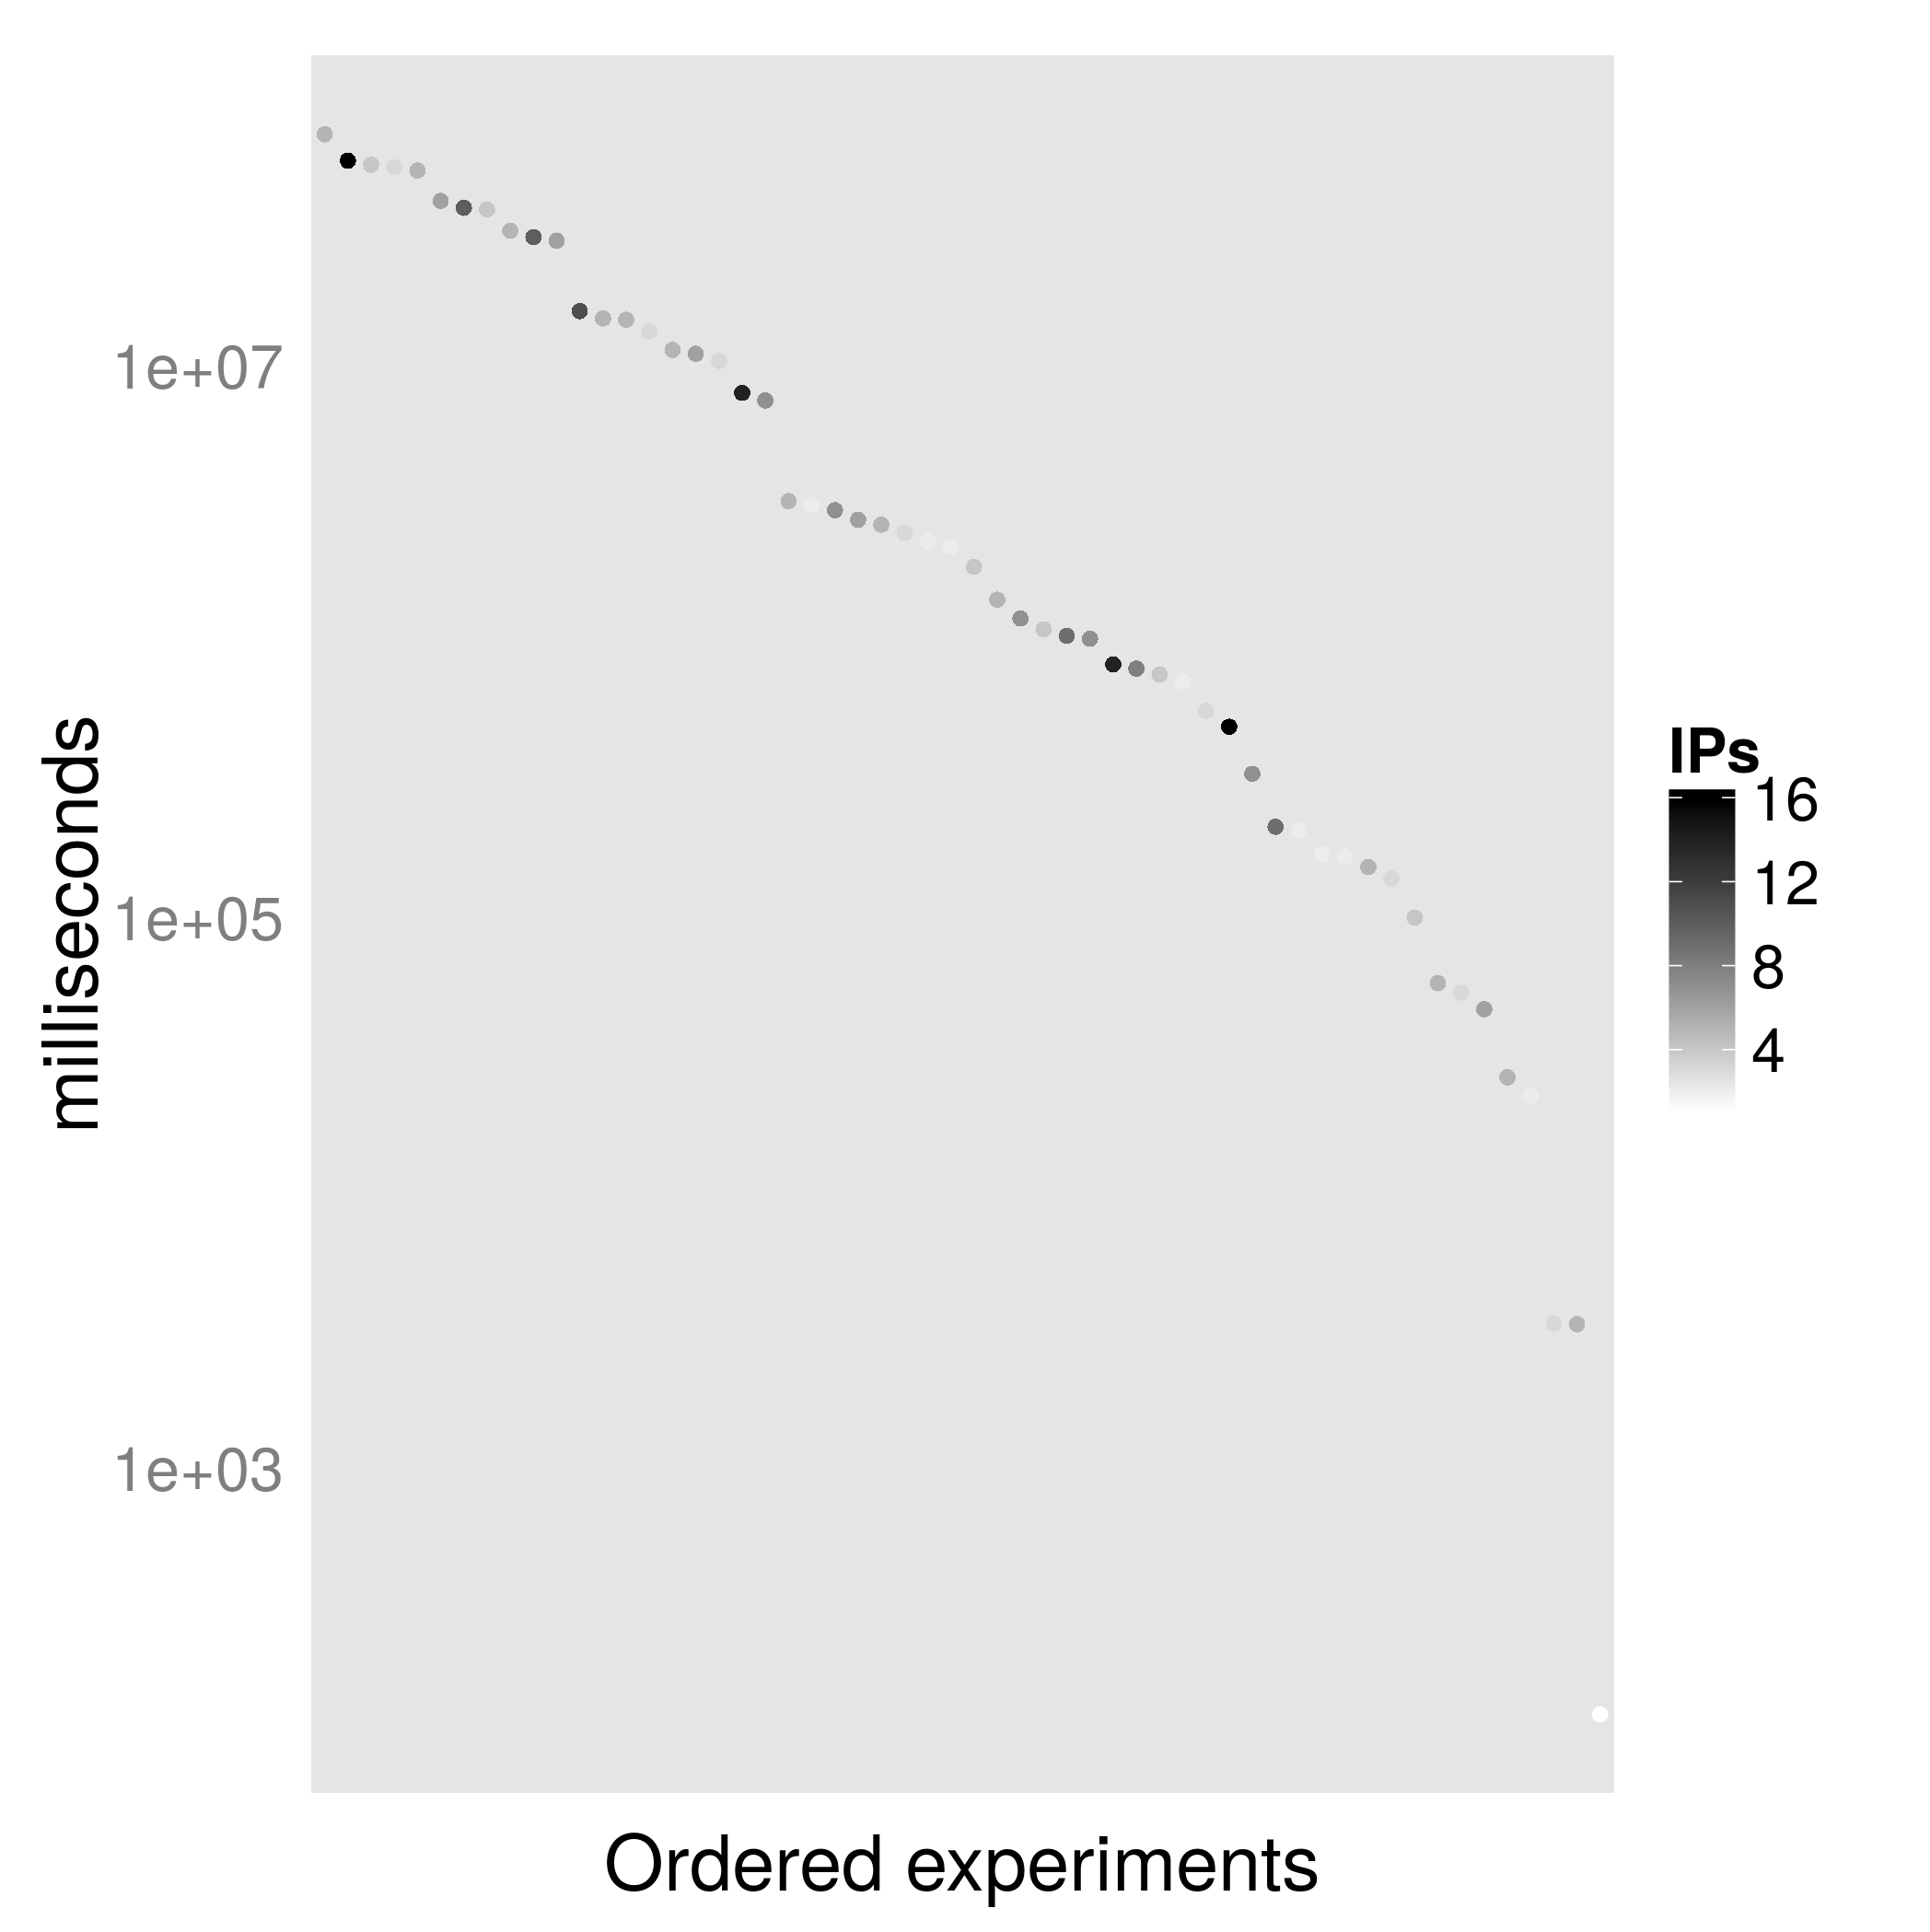
\includegraphics[width=0.32\linewidth]{img/time-vs-rank-OS-4-4.png}
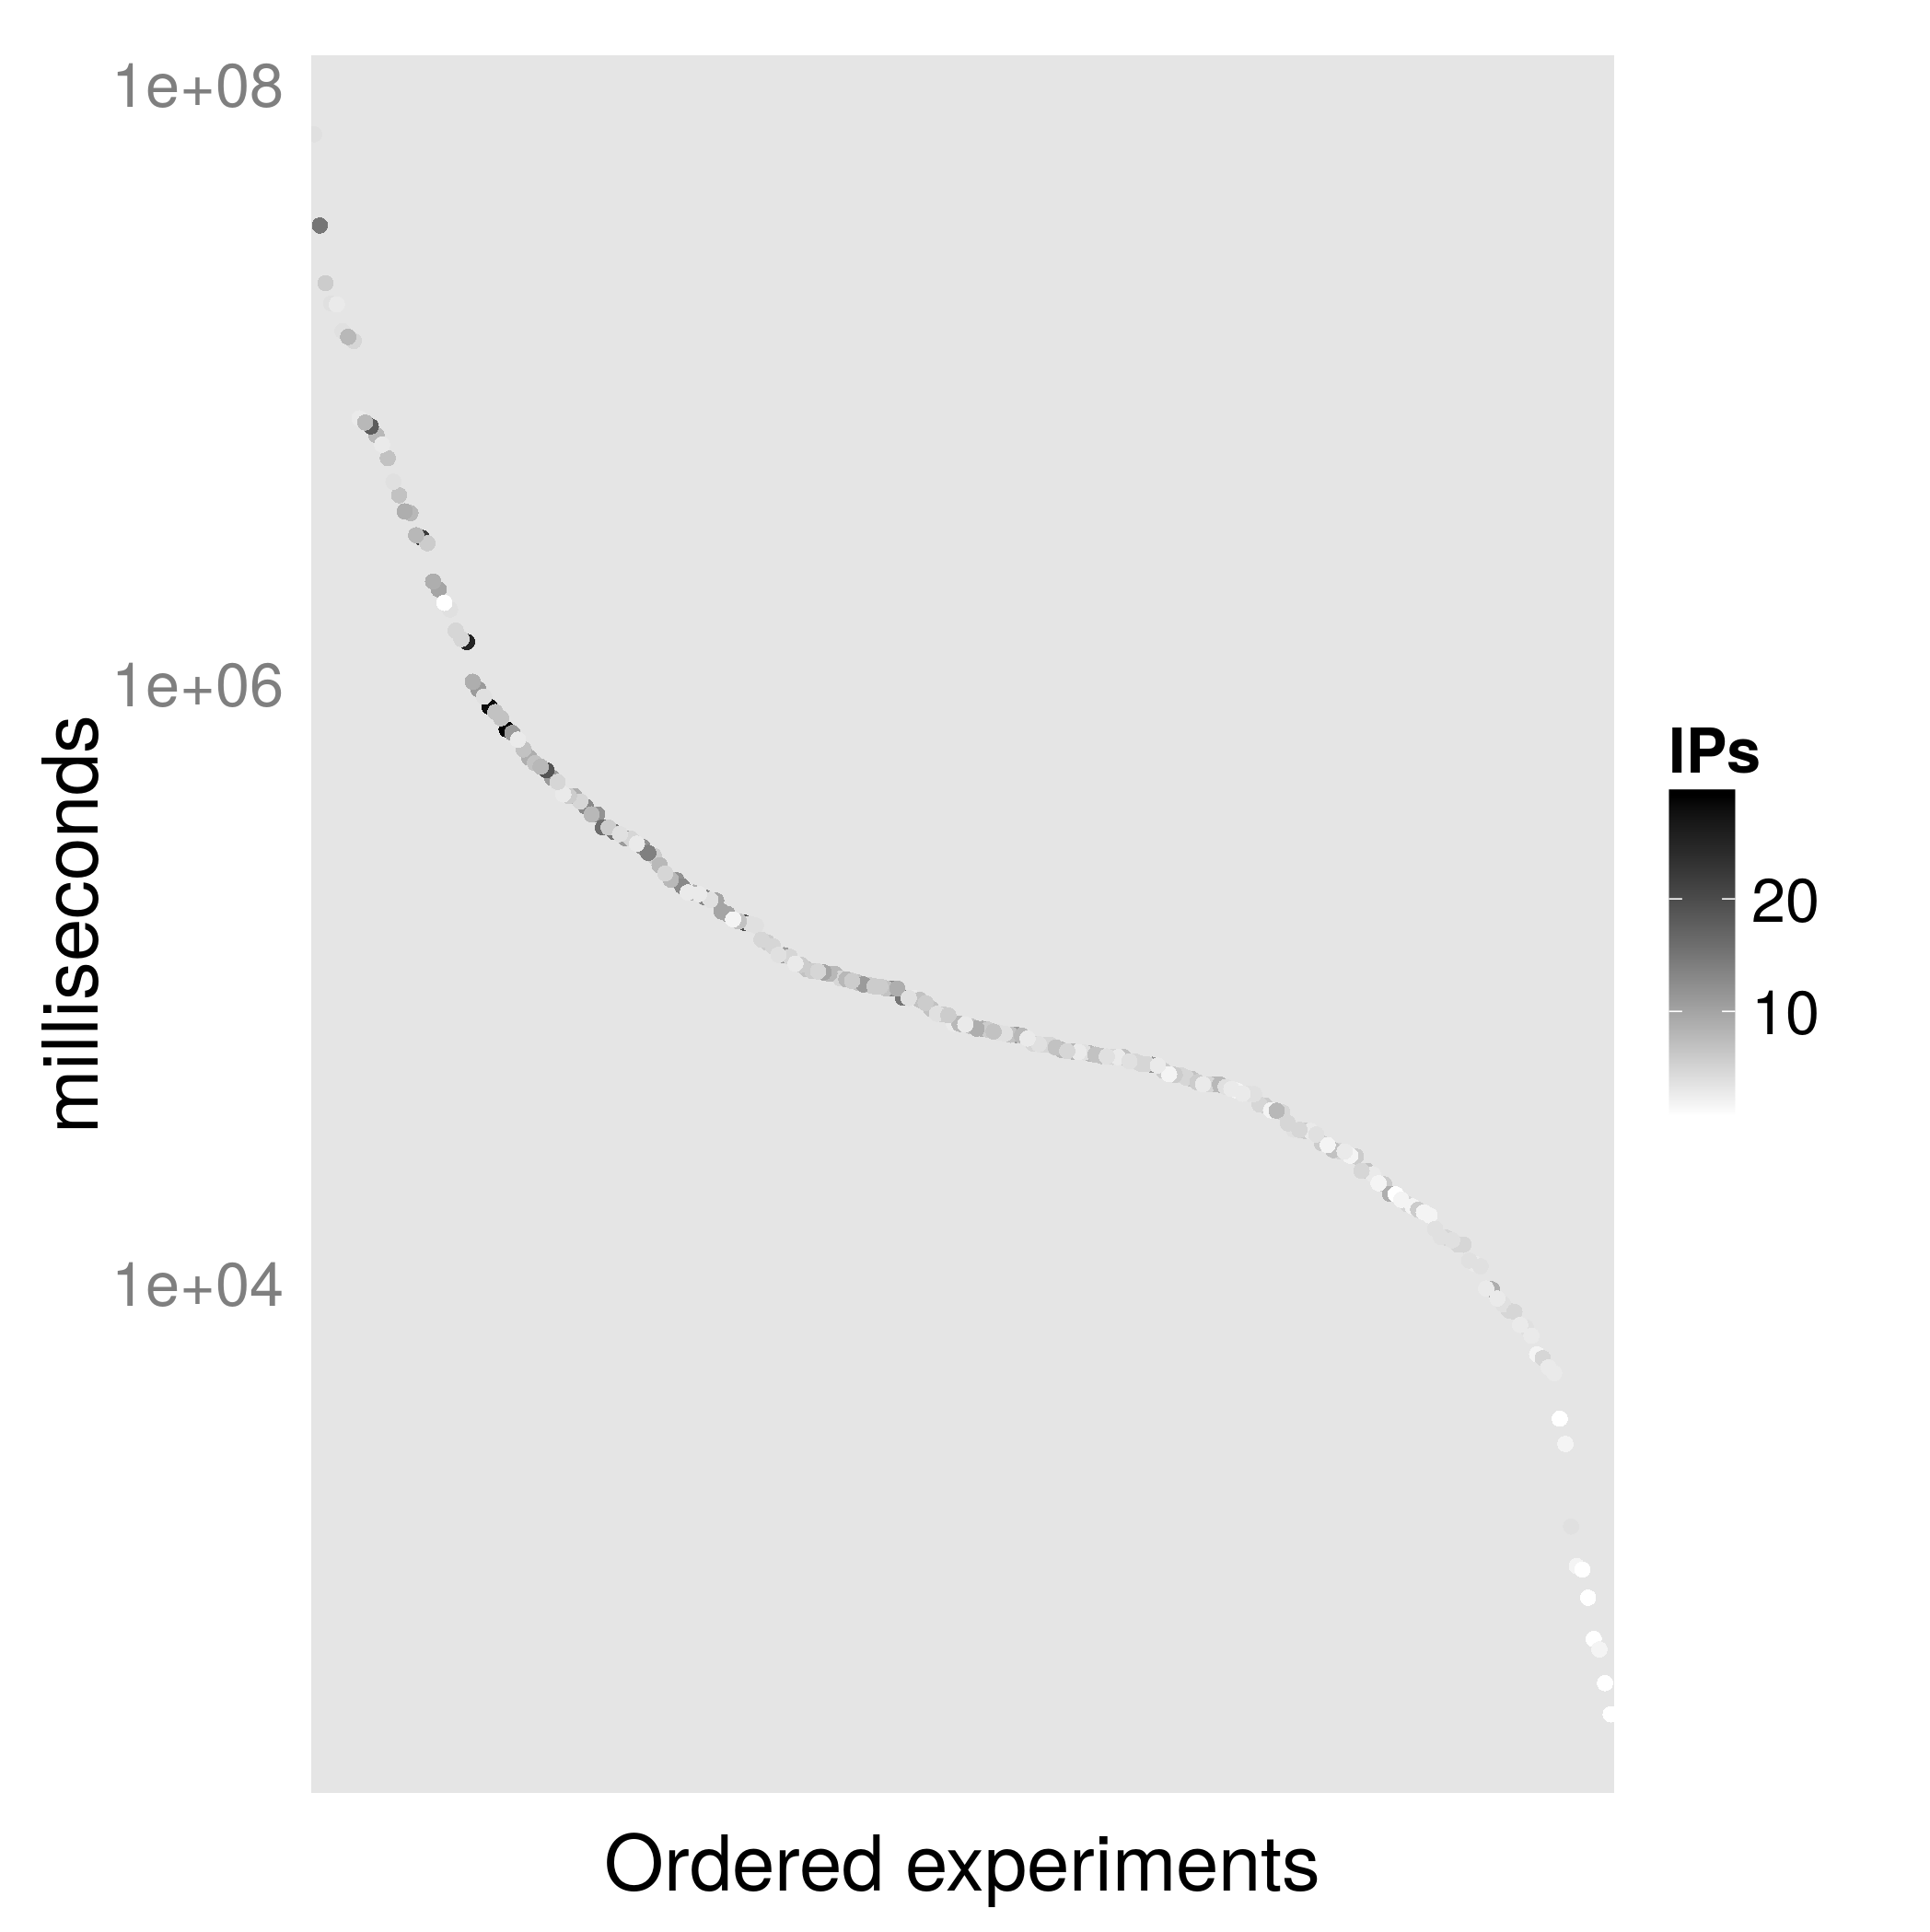
\includegraphics[width=0.32\linewidth]{img/time-vs-rank-OS-4-24.png}
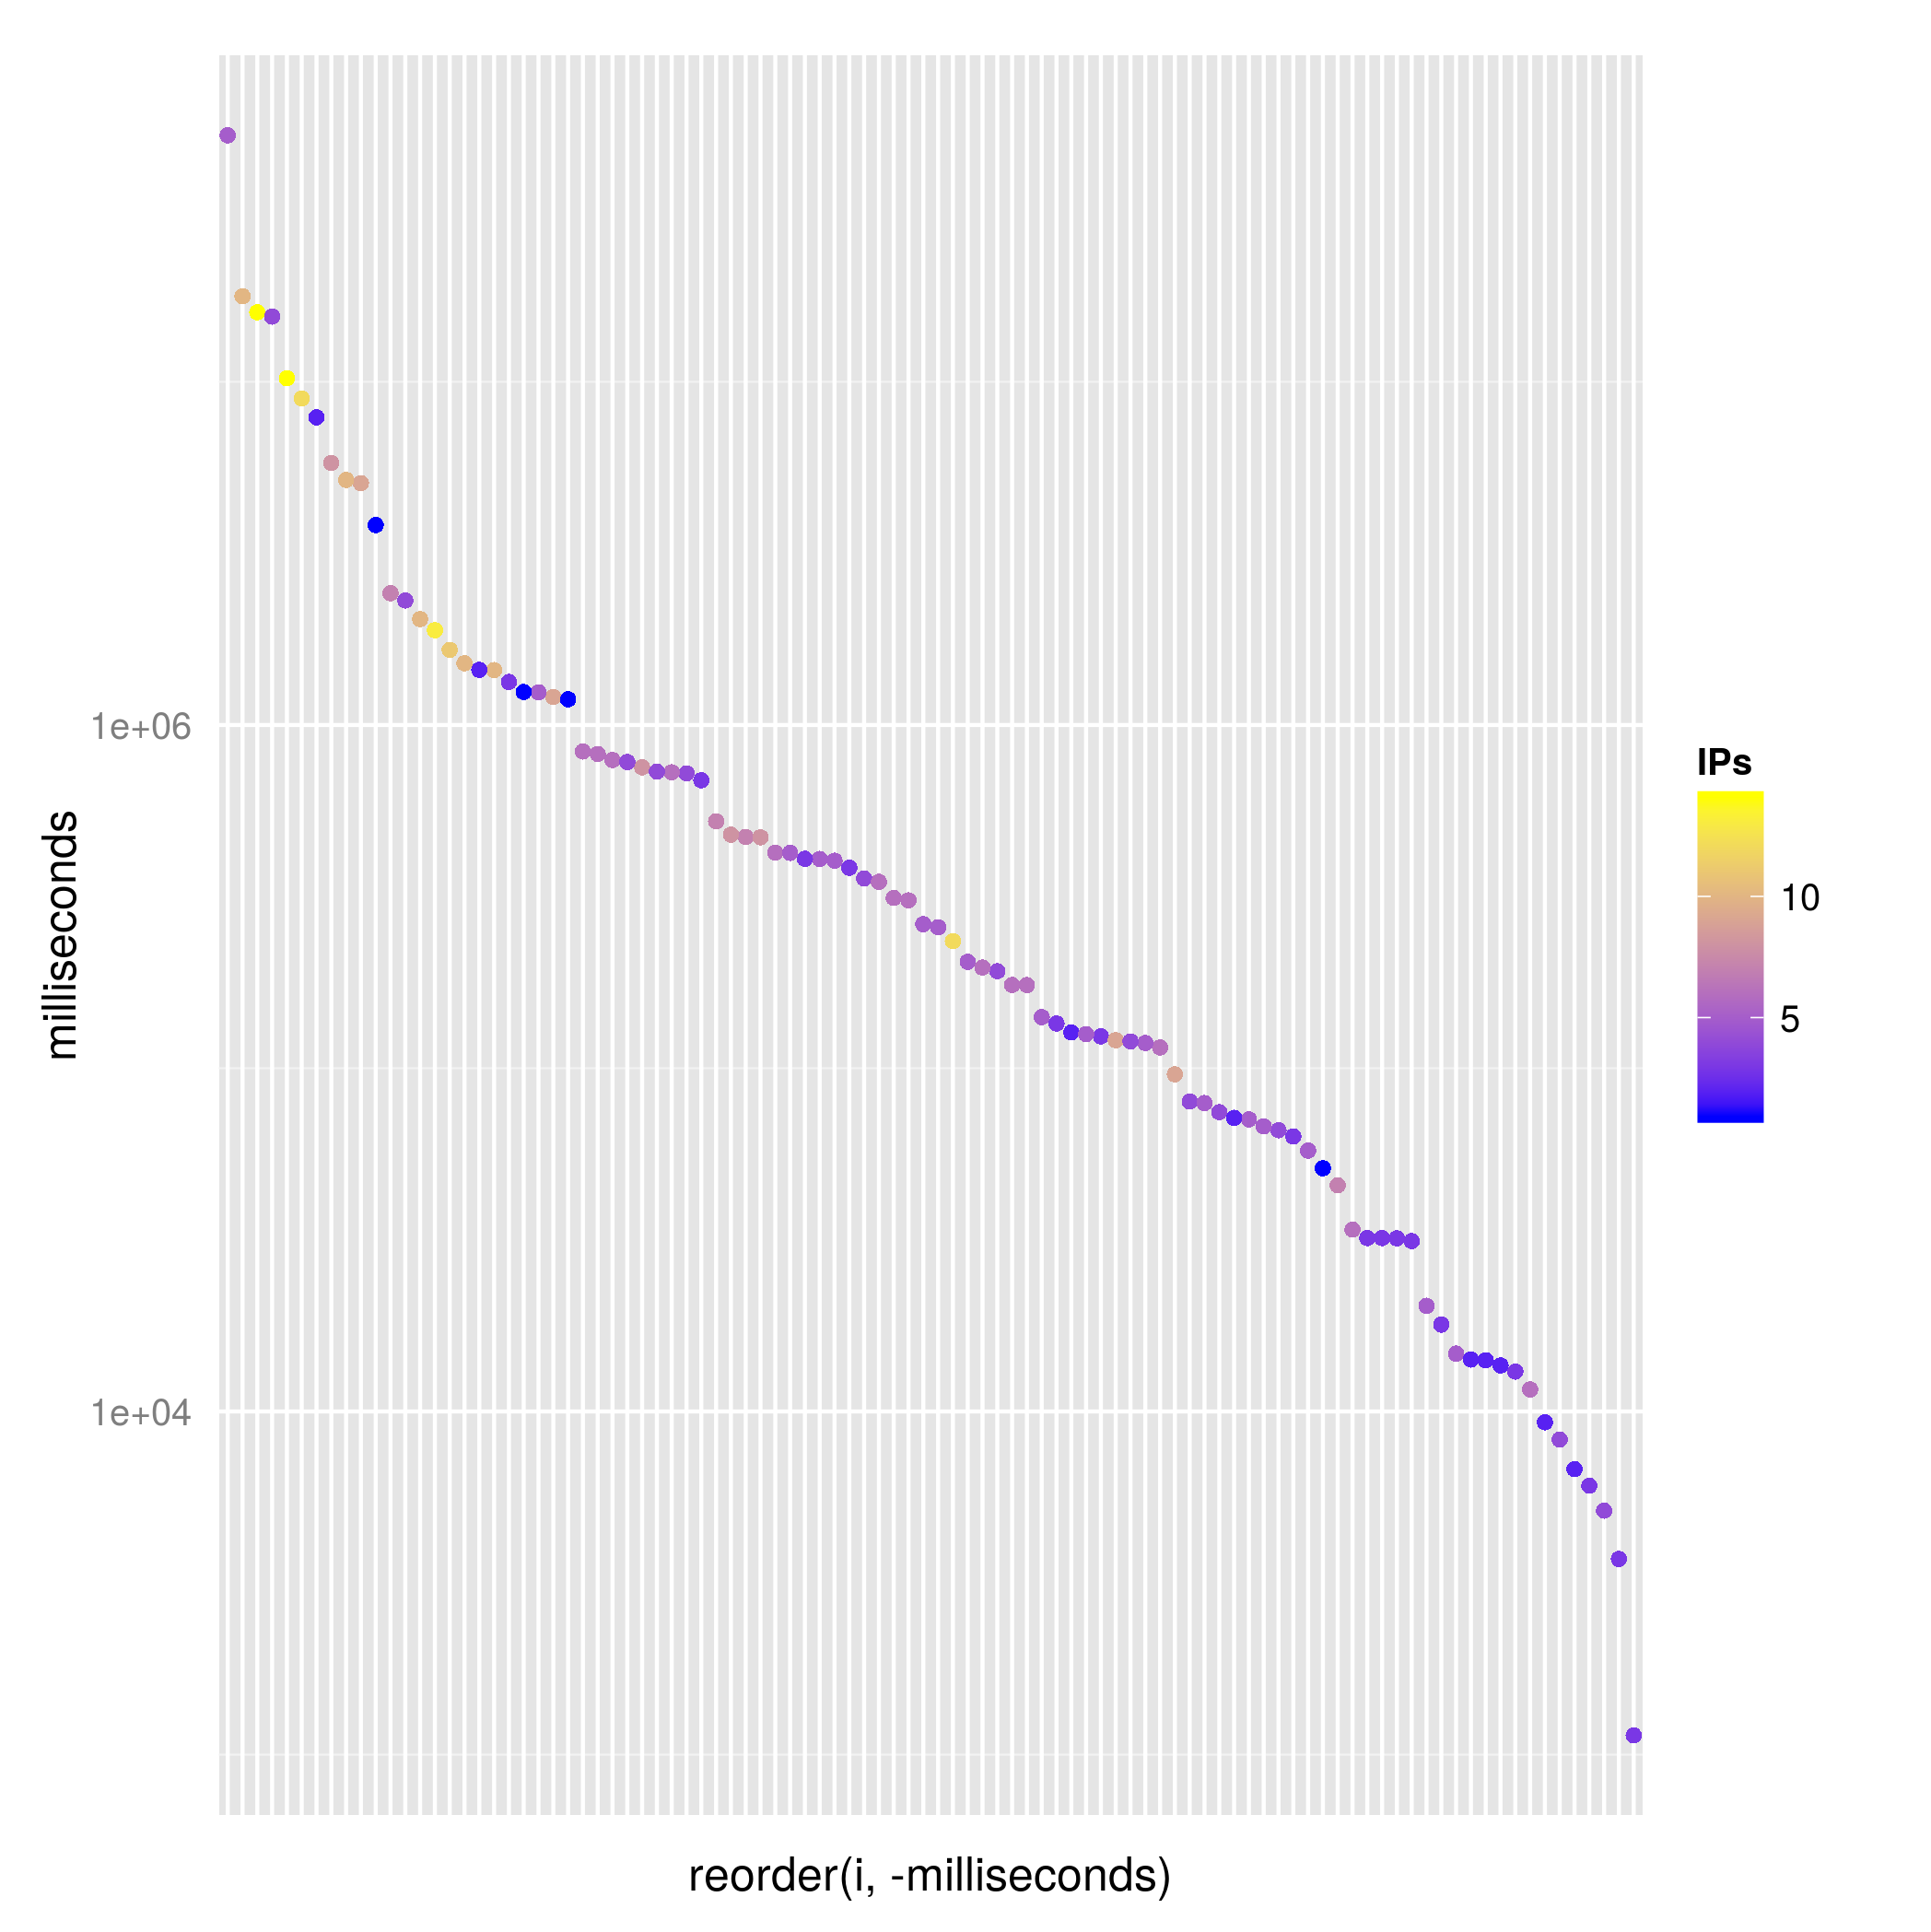
\includegraphics[width=0.32\linewidth]{img/time-vs-rank-OS-7-31.png}
\caption{Duration of experiments vs. rank, with $y$ axis in a
  logarithmic scale. Dot color is related to the number of IPs
  participating in the experiment. From left to right, experiments
  4/4, 4/24 and 7/31.} 
\label{fig:zipf:os}
\end{figure}
%
We will have to analyze experiment data a bit further to find out why
this happens and also if there are some patterns in the three sets of
experiments. An interesting question to ask, for instance, is if
adding more computers makes the experiment take less. In fact, as
shown in Figure \ref{fig:duration}, {\em adding} more computers does
not seem to contribute to decreasing the time needed to finish the
experiment. However, the cause-effect relationship is not clear at
all. It might be the opposite: since experiments take longer to finish
and might in fact be abandoned with no one contributing for some time,
that increases the probability of someone new joining them. In fact,
with experiments taking a few seconds and due to the way the
experiments are announced, it is quite difficult that several
volunteers join in in such a short period of time, even more so taking
into account that volunteers are not {\em carried over} from previous
experiments. This implies that it would be convenient to use a problem
with a bigger size to check this hypothesis; however, at this point we
have not found this convenient since there are several other issues
that have to be solved, as it will be shown next. %FERGU: and that
                                %will be explained next? Algún
                                %ejemplo? 
% A ver si así - JJ

\begin{figure}[!htb]
\centering
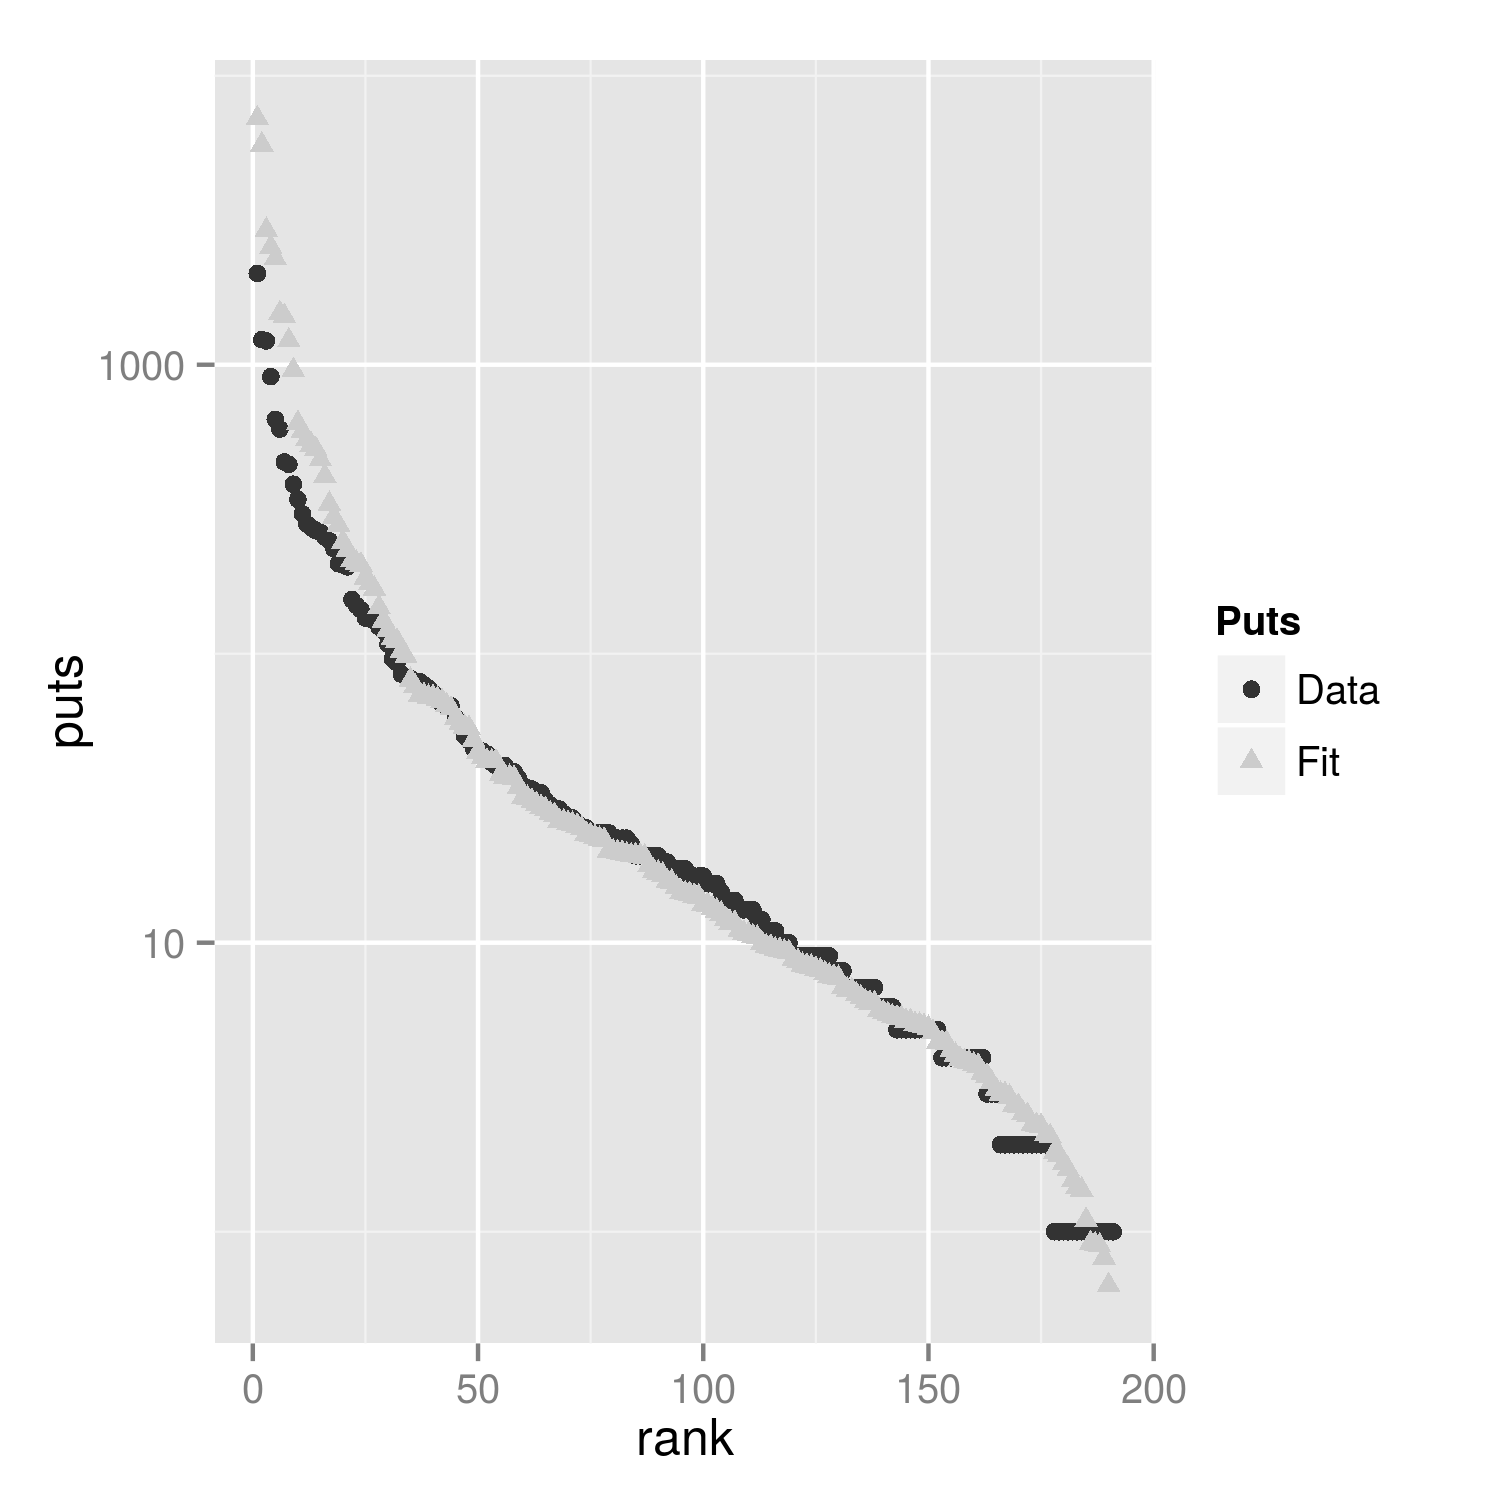
\includegraphics[width=0.32\linewidth]{img/puts-openshift-4-4.png}
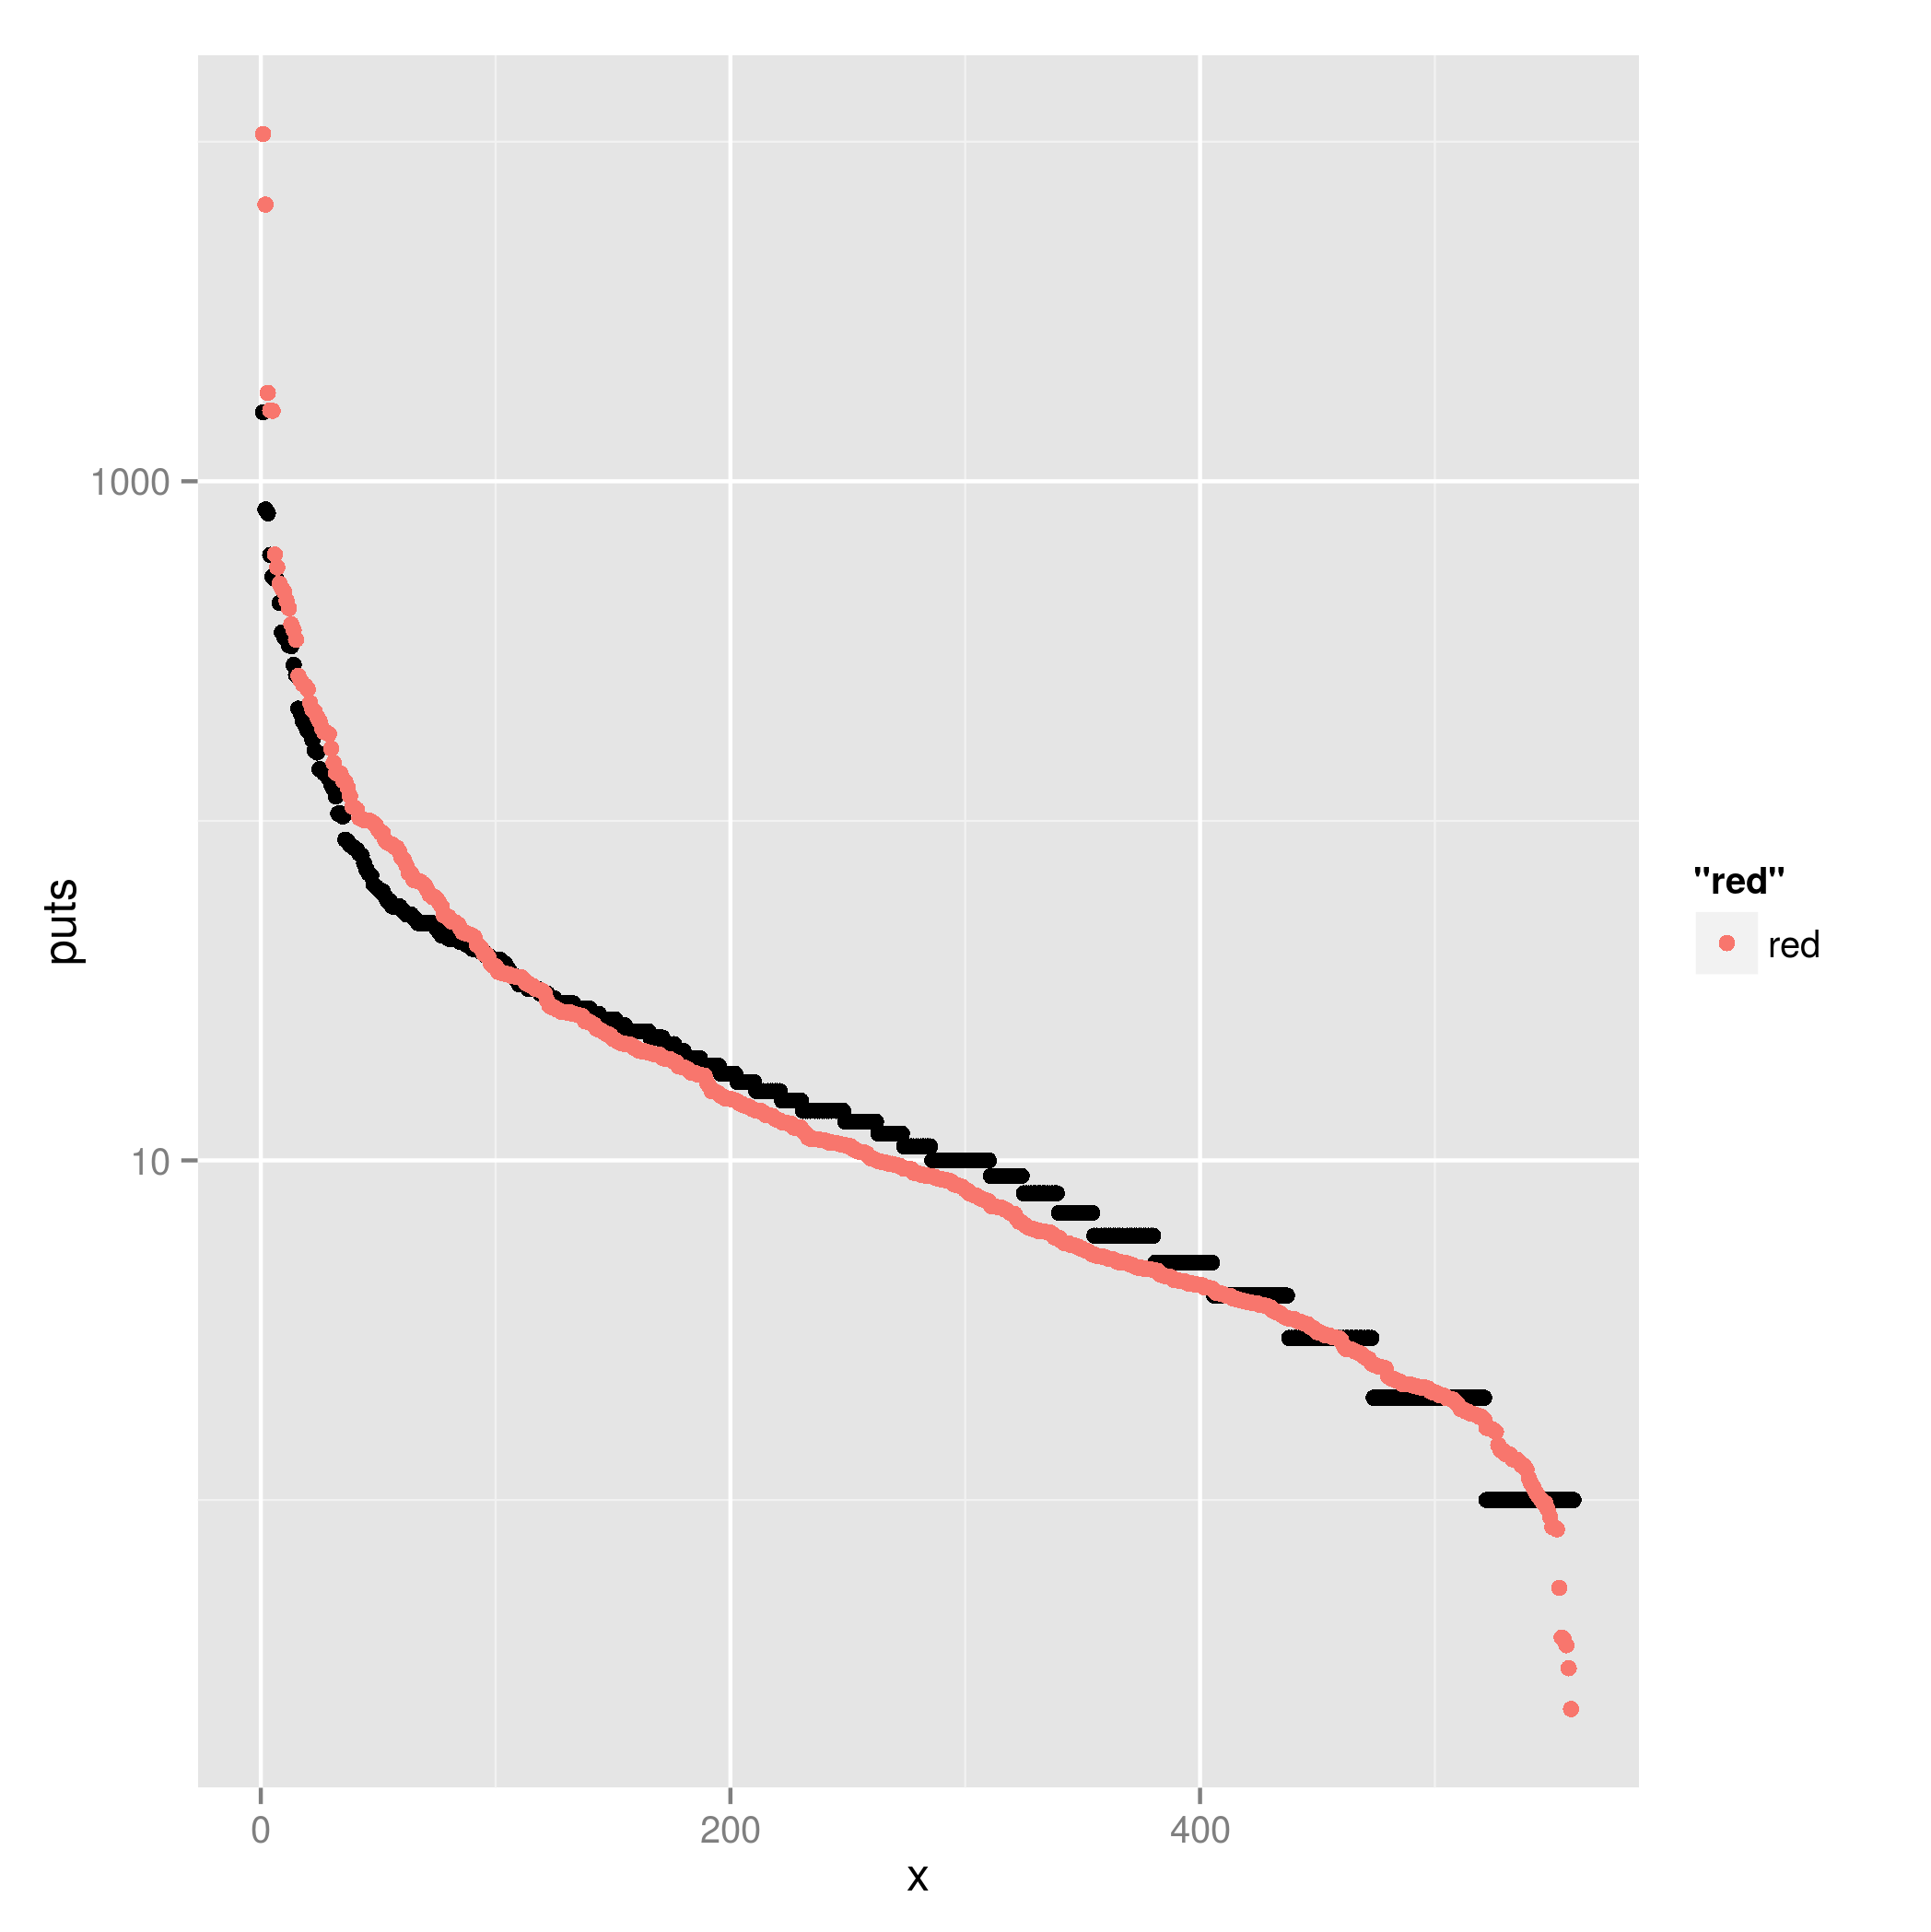
\includegraphics[width=0.32\linewidth]{img/puts-openshift-4-24.png}
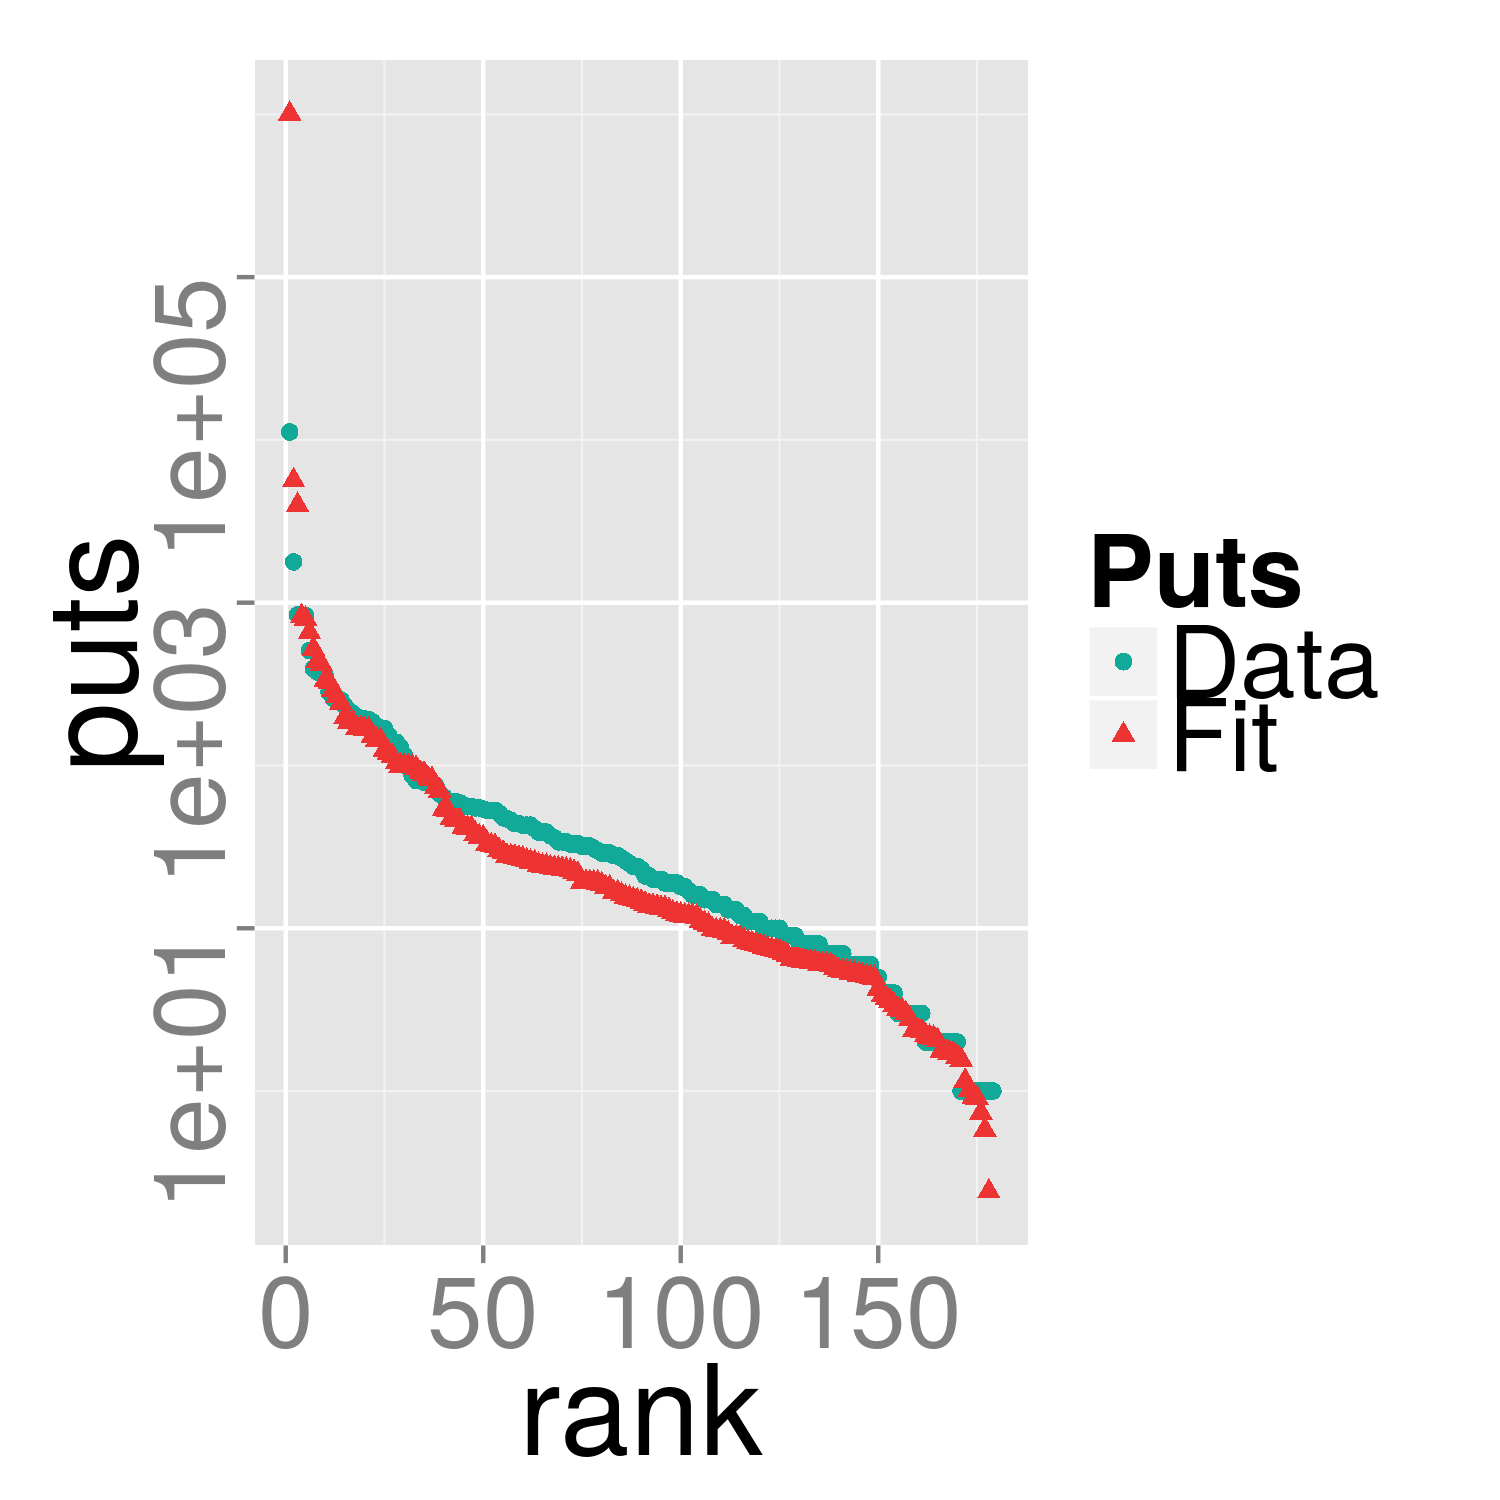
\includegraphics[width=0.32\linewidth]{img/puts-openshift-7-31.png}
\caption{Number of {\tt PUT}s per unique IP and fit to a Generalized
  Extreme Value distribution (in red). From left to right, experiments
  4/4, 4/24 and 7/31.} 
\label{fig:puts:os}
\end{figure}
%

It is interesting also to check the distribution of the experiment
duration, shown in Figure \ref{fig:zipf:os} and which roughly follows
a Zipf's law, with similar distribution along all three runs. The 4/24
run is the most complete and shows a S-shape, which implies an
accumulation of experiments taking similar time and around 100
seconds. The most interesting part is the {\em tail}, which shows how
many experiments took a desirable amount of time, and of the order of
10 seconds. As it can be seen, it drops sharply implying there are
just a few of them, and with diminishing probability as time
decreases. This exponential distribution also appears in the
distribution of HTTP {\tt PUT}s, equivalent to the number of
generations divided by 100, contributed by every user, which is shown
in Figure \ref{fig:puts:os}. These results show a Zipf-like behavior,
so we have fitted it to the Generalized Extreme Value distribution,
with the resulting parameters shown in Table \ref{tab:puts:os}.
%
\begin{table*}
\caption{Summary of fit to Generalized Extreme Value distribution of
  the number of {\tt PUT}s per unique IP. \label{tab:puts:os}}
\begin{center}
\begin{tabular}{l|ccc}
\hline
Date  & Location $\mu$ & Scale $\sigma$ & Shape $\xi$ \\
\hline
4/4 &  8.541 $\pm$ 1.0926  &    12.442 $\pm$ 1.7302 &  1.388 $\pm$
0.1377 \\
4/24 & 6.148 $\pm$ 0.3782 & 7.354 $\pm$ 0.5105 & 1.090 $\pm$  0.0697  \\
7/31 & 11.645 $\pm$ 1.475 & 16.365 $\pm$ 2.201 &  1.265 $\pm$ 0.132   \\
\hline
\end{tabular}
\end{center}
\end{table*}
%
This distribution was originally proposed to fit extreme values
\cite{resnick2013extreme} and contains, as a special case, the inverse
Weibull distribution which was fitted to volunteer computing
frameworks such as SETI@home \cite{javadi2009mining}. This
distribution is governed by three parameters, the usual location $\mu$
which is related to where it has its {\em center} and  scale $\sigma$,
related to the size, but also a third shape $\xi$ parameter that is
related to its skewness, that is, how skewed it is around the central
location. Positive parameters indicate that the distribution {\em
  leans} towards the origin, negative towards the other extreme
value. In this case, Table \ref{tab:puts:os} shows $\xi$ values
greater than one and between one and 1.4, which indicates that the
three experiments share this origin-leaning pattern, with many users
donating a few cycles and just a few donating extreme values. Random
distributions with these parameters have been plotted in red in
Figure \ref{fig:puts:os}, indicating that the fit is good enough. The
predictive value of these fits, however, is limited, over all taking
into account the low correlation between successive events shown
above.

At any rate, this also shows that a convenient way of increasing the
computing power would be increasing this minimum amount per user. This
issue led us to create the next version of the framework, which is
presented next. %Fergu: esto mola, métele más caña en otras secciones
                %para que se vea que es una conclusión util 
% Está en las conclusiones - JJ

\subsection{{\sf NodIO-W$^2$}, a Web Worker-based architecture}

In order to improve the number of cycles per user, we improved the
basic architecture in several different aspects. By using Web Workers %FERGU: WebWorker separado o junto? homogeneizar
the algorithm kept running on the background even if the {\sf NodIO}
tab was not in focus. It also allowed to run several clients per
browser, as opposed to a single one as we did previously. Another
improvement involved restart of the client once the solution was
found, so that as long as the user was visiting the page it was
running an evolutionary algorithm. Finally, a small algorithmic
improvement was included: instead of having a fixed population,
population size was random and different for each client. %FERGU: mínimo y máximo?

JavaScript has been commonly used to develop client-side scripts
that handle the user interface, communicate asynchronously with servers and
update the content that is displayed \cite{flanagan2006javascript}.
Long-running scripts like those proposed in this work can interfere with the
responsiveness of the web application, because everything is handled by a
single thread. The Web Workers specification \cite{hickson2012web} defines an
API that allows Web developers to execute long-running scripts in parallel
with the scripts of the main page. Worker scripts are spawned in the
background allowing a thread-like operation using message-passing as the
communication mechanism between the worker's execution environment and the
main thread. According to the Web Workers W3C Candidate Recommendation
\cite{hickson2012web} workers are expected to be long-lived, they have a high
start-up performance cost, and a high per-instance memory cost. The Web Worker
API is implemented in current versions of both desktop and mobile web browsers.
For volunteer computing using the Web Worker API brings several advantages
over a single threaded implementation:

\begin{itemize}
\item If the browser uses a tabbed document interface, the worker script
keeps running in the background even it the user brings forward another tabbed
window.
\item Several evolutionary algorithms can be executed in parallel in a single web
page. %FERGU: NodEO o NodIO? (es NodEO la instancia, creo pero por si
      %acaso :P)
% Mejor evolutionary algorithms - JJ
\item Many implementations of the Web Worker API can use multiple CPUs for
the execution of worker scripts, in particular the execution in multiple CPUs
was tested in desktop versions of Chrome, FireFox and Safari.
\item Each NodEO instance can be restarted independently.
\end{itemize}

A sequence diagram of the W$^2$ version of {\sf NodIO} is presented
in Figure~\ref{fig:system:w2}. In this version, clients use the Web Workers
API to run two NodEO instances per browser. The sequence diagram shows the
interaction between processes in a time sequence. In this system there are
two kinds of asynchronous messages: HTTP Requests shown as bold arrows between
the client and the server where PUT and GET HTTP Methods are represented by
red and blue arrows respectively. There are also messages between workers and
the main thread in locally in the client, these are shown as thin solid arrows.
There are three processes involved:
\begin{itemize}
\item {\em nodejs} This is the server side process which is basically
  the same as used previously, except for some minor log-related
  changes. 
\item {\em Client main thread}  This process handles the user interaction
using the JQuery framework. The Chart.js library is used to display a chart of
the best fitness in the population over time. The main script also creates
worker instances and handles the user interface.
\item {\em Worker global scope} The worker execution space does not have
access to the Document Object Model (DOM) or JQuery objects in the main thread.
Asynchronous HTTP requests to the server are implemented using the XHR object. %FERGU: Qué es el objeto XHR? Alguna referencia/justificación de por qué se usa?
\end{itemize}
%
\begin{figure}[!htb]
\centering
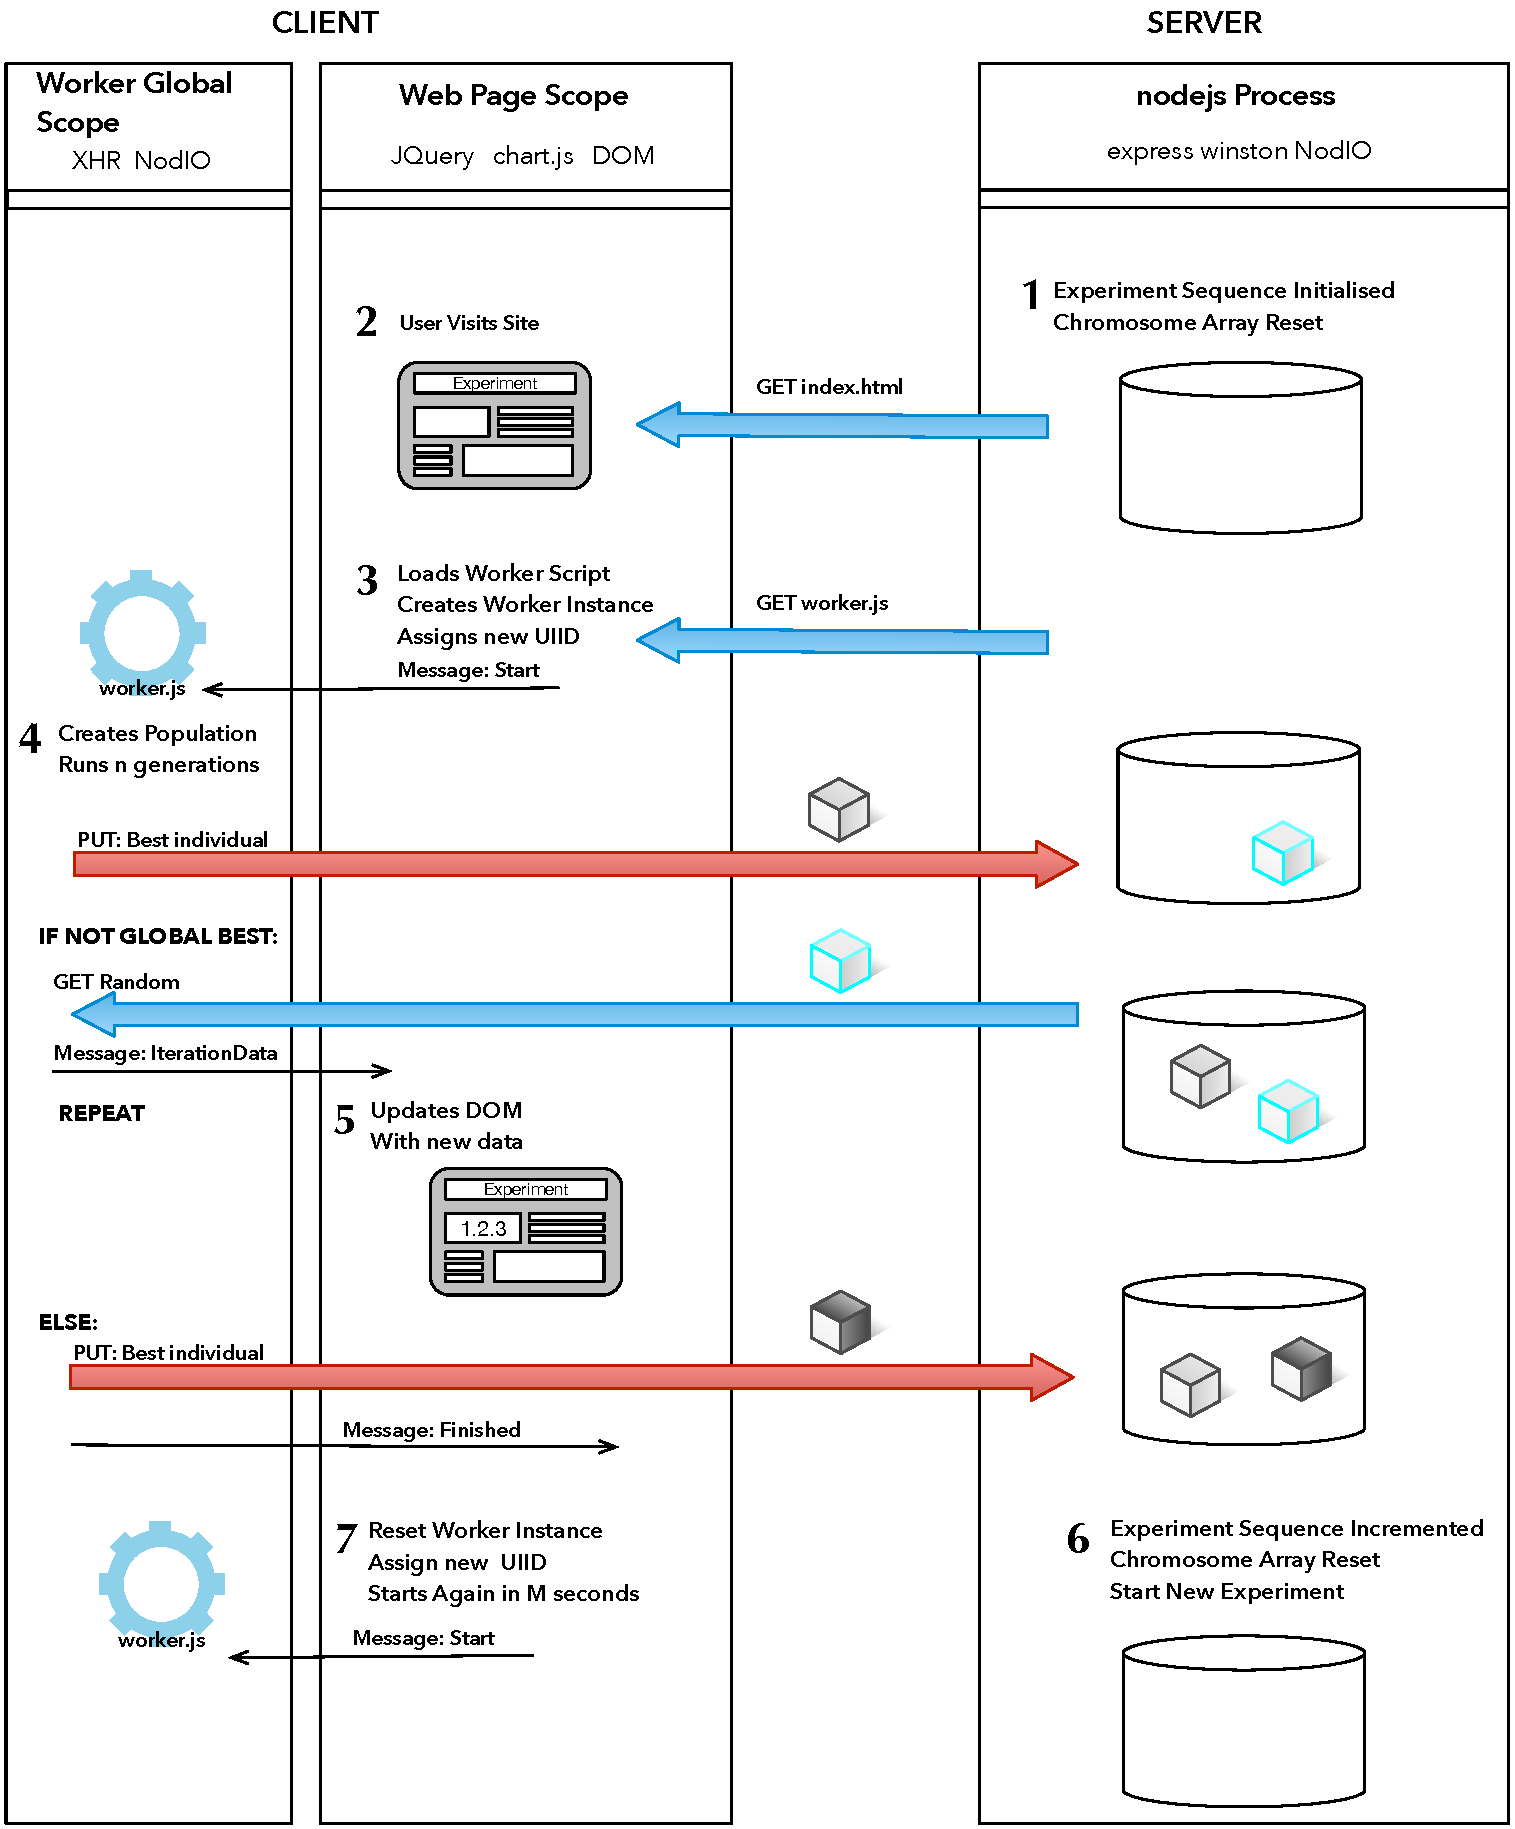
\includegraphics[width=4in]{img/Algorithm.pdf}
\caption{Description of the W$^2$ version of {\sf NodIO}. In this
  version, clients use Web Workers to run the evolutionary algorithm,
  with two of them per browser.}
\label{fig:system:w2}
\end{figure}

The sequence of events is as follows:
\begin{enumerate}
\item First the {\sf NodIO} process is started in nodejs. As part of the
initialization procedure the number of experiment is initialized and a log
file is created. The shared pool implemented as an array is reset.
\item A volunteer follows the link of the experiment triggering a GET HTTP
request and the page is loaded.
\item The main script renders the page and creates the worker instance. In
order to create a dedicated worker instance, another GET request is sent to the
server in order to receive the worker implementation script.
Each worker instance executes one or more evolutionary algorithms
{\em islands}. Each starts with random population and it is assigned a
universally unique  identifier (UUID). The UUID is included in each of the HTTP
requests sent to the server.
The initial parameters for each island
can be distinct. Once the worker is created and the parameters have been set,
a message is sent to the worker to start the algorithm.
\item The worker first creates the population following with the previously
specified parameters. Once the population has been initialized, the EA
generation loop is started. After {\em n} generations the state of the population
is evaluated. First the chromosome with the best fitness is sent to the shared
population with a PUT HTTP request. If the best fitness is not a global best,
the EA loop must continue, but first a chromosome is randomly selected from
the shared population. Also the current generation number and the best
chromosome is sent to the client main thread in order to update the DOM to
display the current state of the island (described next). These messages are
all asynchronous, so even before a message is received by target the EA loop of
the worker could continue. If the best fitness is a global best the best
chromosome is sent to the server and the loop ends. A message is sent to the
main thread indicating that the best individual has been found.
\item The main thread receives messages from workers as events handled by
a callback function. When an iteration message is received, the page is
updated by displaying a dynamic plot of the generation number and best
fitness, and a representation of the chromosome is also generated.
\item When a global best is received from an island the current experiment
ends, the experiment number is incremented and the population array is reset.
\item When the main thread receives a message the a worker has ended the EA
loop, that worker is reinitialized. The worker process is not ended, to
avoid the cost, only the parameters and population is reset and a new UIID
assigned.
\end{enumerate}
%
\begin{table*}[!htb]
\caption{Summary of {\sf NodIO-W$^2$} and comparison with the previous
  experiments, which have been aggregated to compute central measures. \label{tab:summary:ww}}
\begin{center}
\begin{tabular}{l|ccccccc}
\hline
Date & Median \#IPs & Max \#IPs & Median time (s) & Median \#{\tt
  PUT}s & $<$ 69s & $<$ 3.46s & Inter-experiment correlation\\
\hline
{\sf NodIO} & 5 & 29 & 123 & 14 & 37.43\% & 3.40\% & 0.10 \\
{\sf NodIO-W$^2$} & 4  & 16 & 7.36 & 40 & 89\% & 36.90\% & 0.4336061 \\
\hline
\end{tabular}
\end{center}
\end{table*}
%

The experiments were run in the same way as before, using several
Twitter announcements throughout several days by the end of July
2015. Eventually, more than one thousand experiments were completed in
a matter of days. A summary of results is shown in Table
\ref{tab:summary:ww}, comparing it with the aggregate of the results
obtained with the initial version of {\sf NodIO}. These results are
remarkably different, being similar only in the median and maximum
number of IPs, although in this case it would be combination
IP-worker, being considered every worker a different IP. The median
number of seconds is almost 80\% better than the previous version, and
the median number of PUTs is three times better; this causes that most
of experiments take less time than one of the baselines, and one third
less than the second baseline. Thus, the conclusion in this case is
that we can obtain, through volunteer computation, a result that is,
most of the times, better than we would using a similar, non-parallel,
desktop setup, which makes this system suitable for massively
distributed evolutionary algorithms.

%FERGU: a lo mejor algún reviewer se queja de que la comparativa no es justa
%porque comparamos un mono-isla (el baseline) con un multi-isla. Quizás deberíamos
%haber usado un multi-isla en el baseline (aunque sea secuencial). Para la próxima.

However, it is interesting to note why this is so, and the first hint
is the inter-experiment correlation between the number of IPs in
successive experiments. While before it was an unremarkable 10\%, it is
now more than 43\%, making the number of IPs in contiguous experiments
highly correlated. The main reason for this is the setup in {\sf
  NodIO-W$^2$}, which restarts an island after a solution has been
found and also is running even if the tab is not on the
foreground. This means that volunteers can leave the experiment
running for as long as they want and they will be contributing to
experiment after experiment, unlike the previous version, where they
stopped contributing after the solution was found. This is also
reflected in the number of PUTs, which is the number of generations
divided by 100; more than 50\% of the volunteers run for more than
4000 generations. All things considered, this means than there are
many more computers running {\em simultaneously}, leading to this
almost 5-fold increase in running time.

\begin{figure}[!htb]
\centering
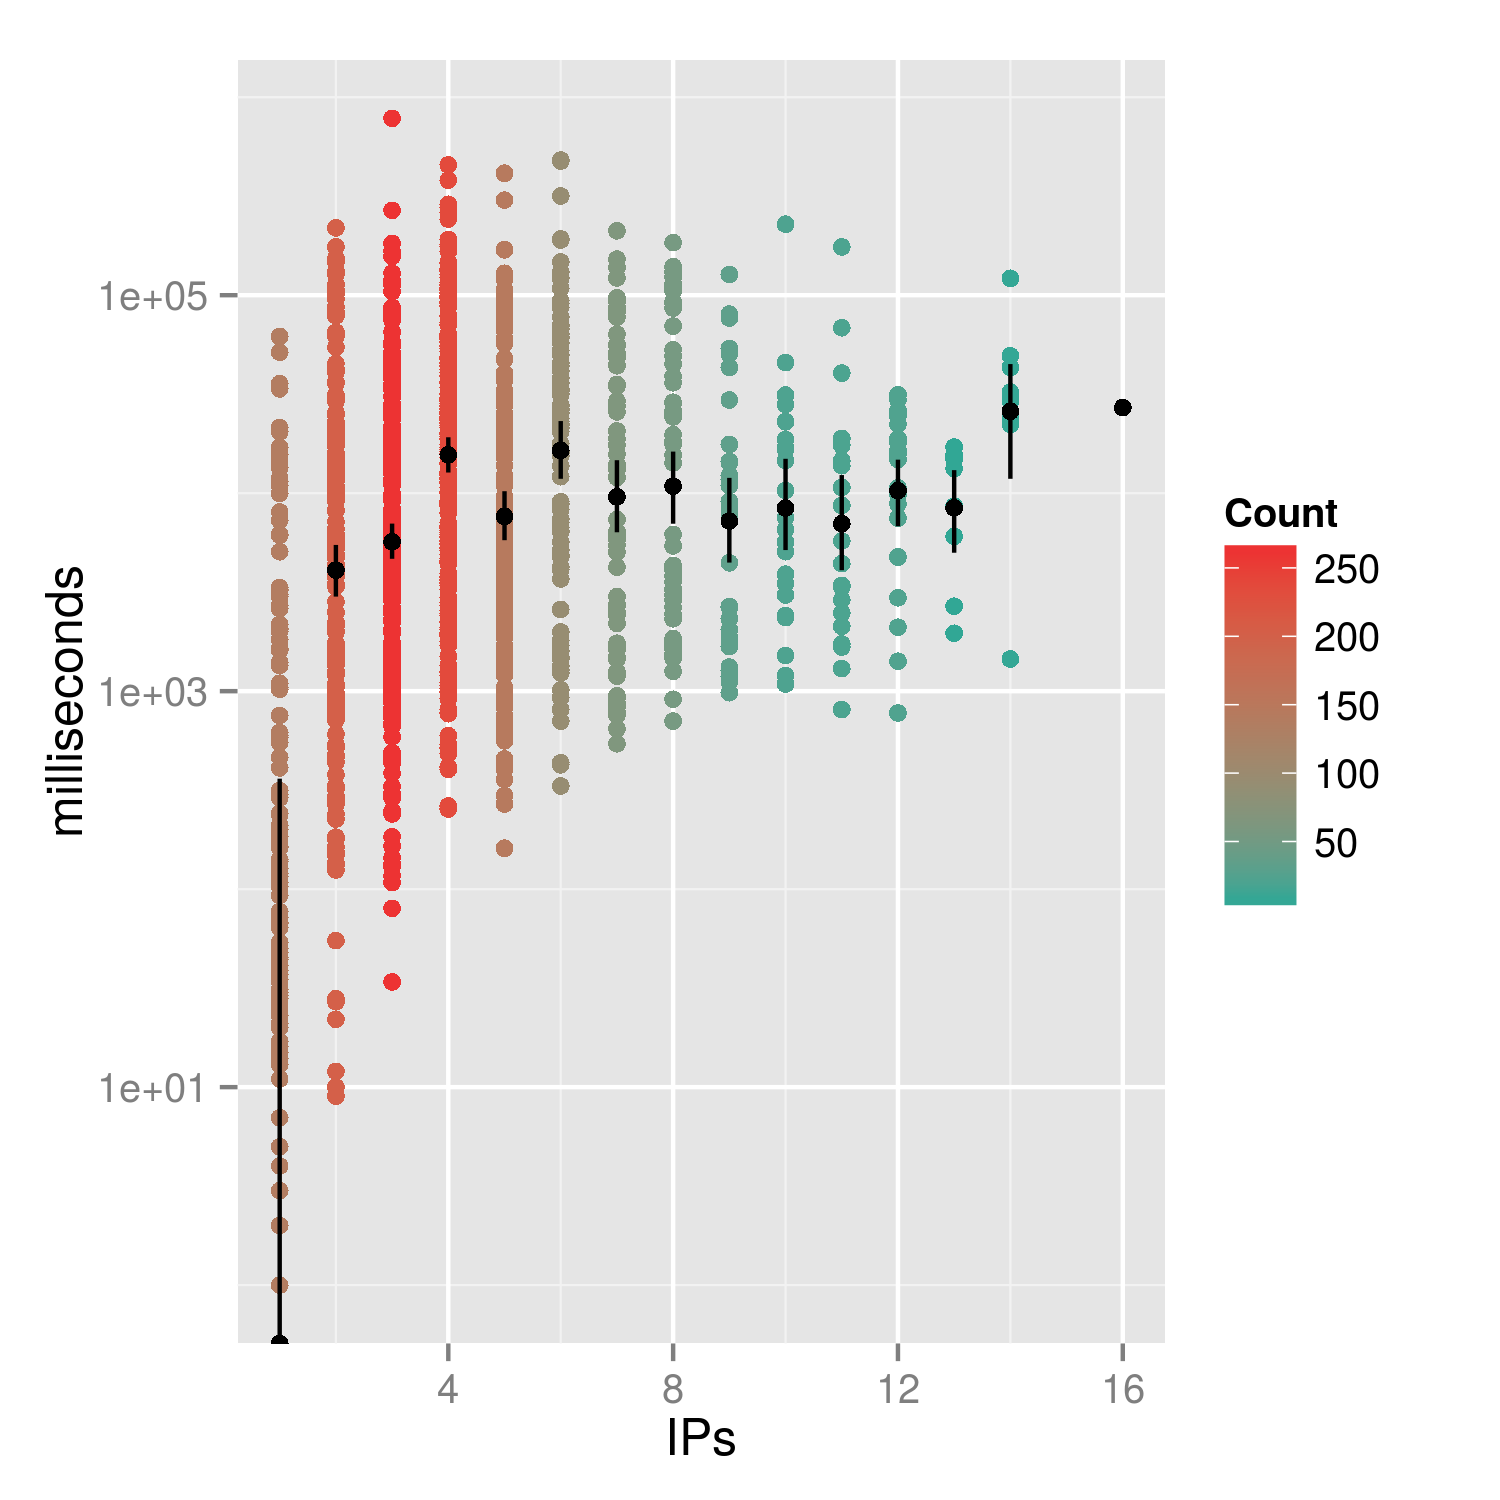
\includegraphics[width=0.9\linewidth]{img/ips-time-ww.png}
\caption{Time employed in every experiment vs. number of IPs (in abscises). The red dot and line show the average and standard deviation, the shade of blue the number of experiments with the same number of IPs. }
\label{fig:ipstime:w2}
\end{figure}
%
%
\begin{table*}
\caption{Summary of fit to Generalized Extreme Value (GEV) and Weibull distribution of
  the number of {\tt PUT}s per worker. \label{tab:puts:ww}}
\begin{center}
\begin{tabular}{cccc}
\hline
Distribution & Location $\mu$ & Scale $\sigma$ & Shape $\xi$ \\
\hline
GEV & 18.275 $\pm$ 0.83719  &  25.962  $\pm$ 1.22015 & 1.242   $\pm$
0.04746 \\
Weibull & ND & 75.11457519 $\pm$ 2.97470251  & 0.69714410 $\pm$ 0.01383976 \\
\hline
\end{tabular}
\end{center}
\end{table*}
%
\begin{figure}[!htb]
\centering
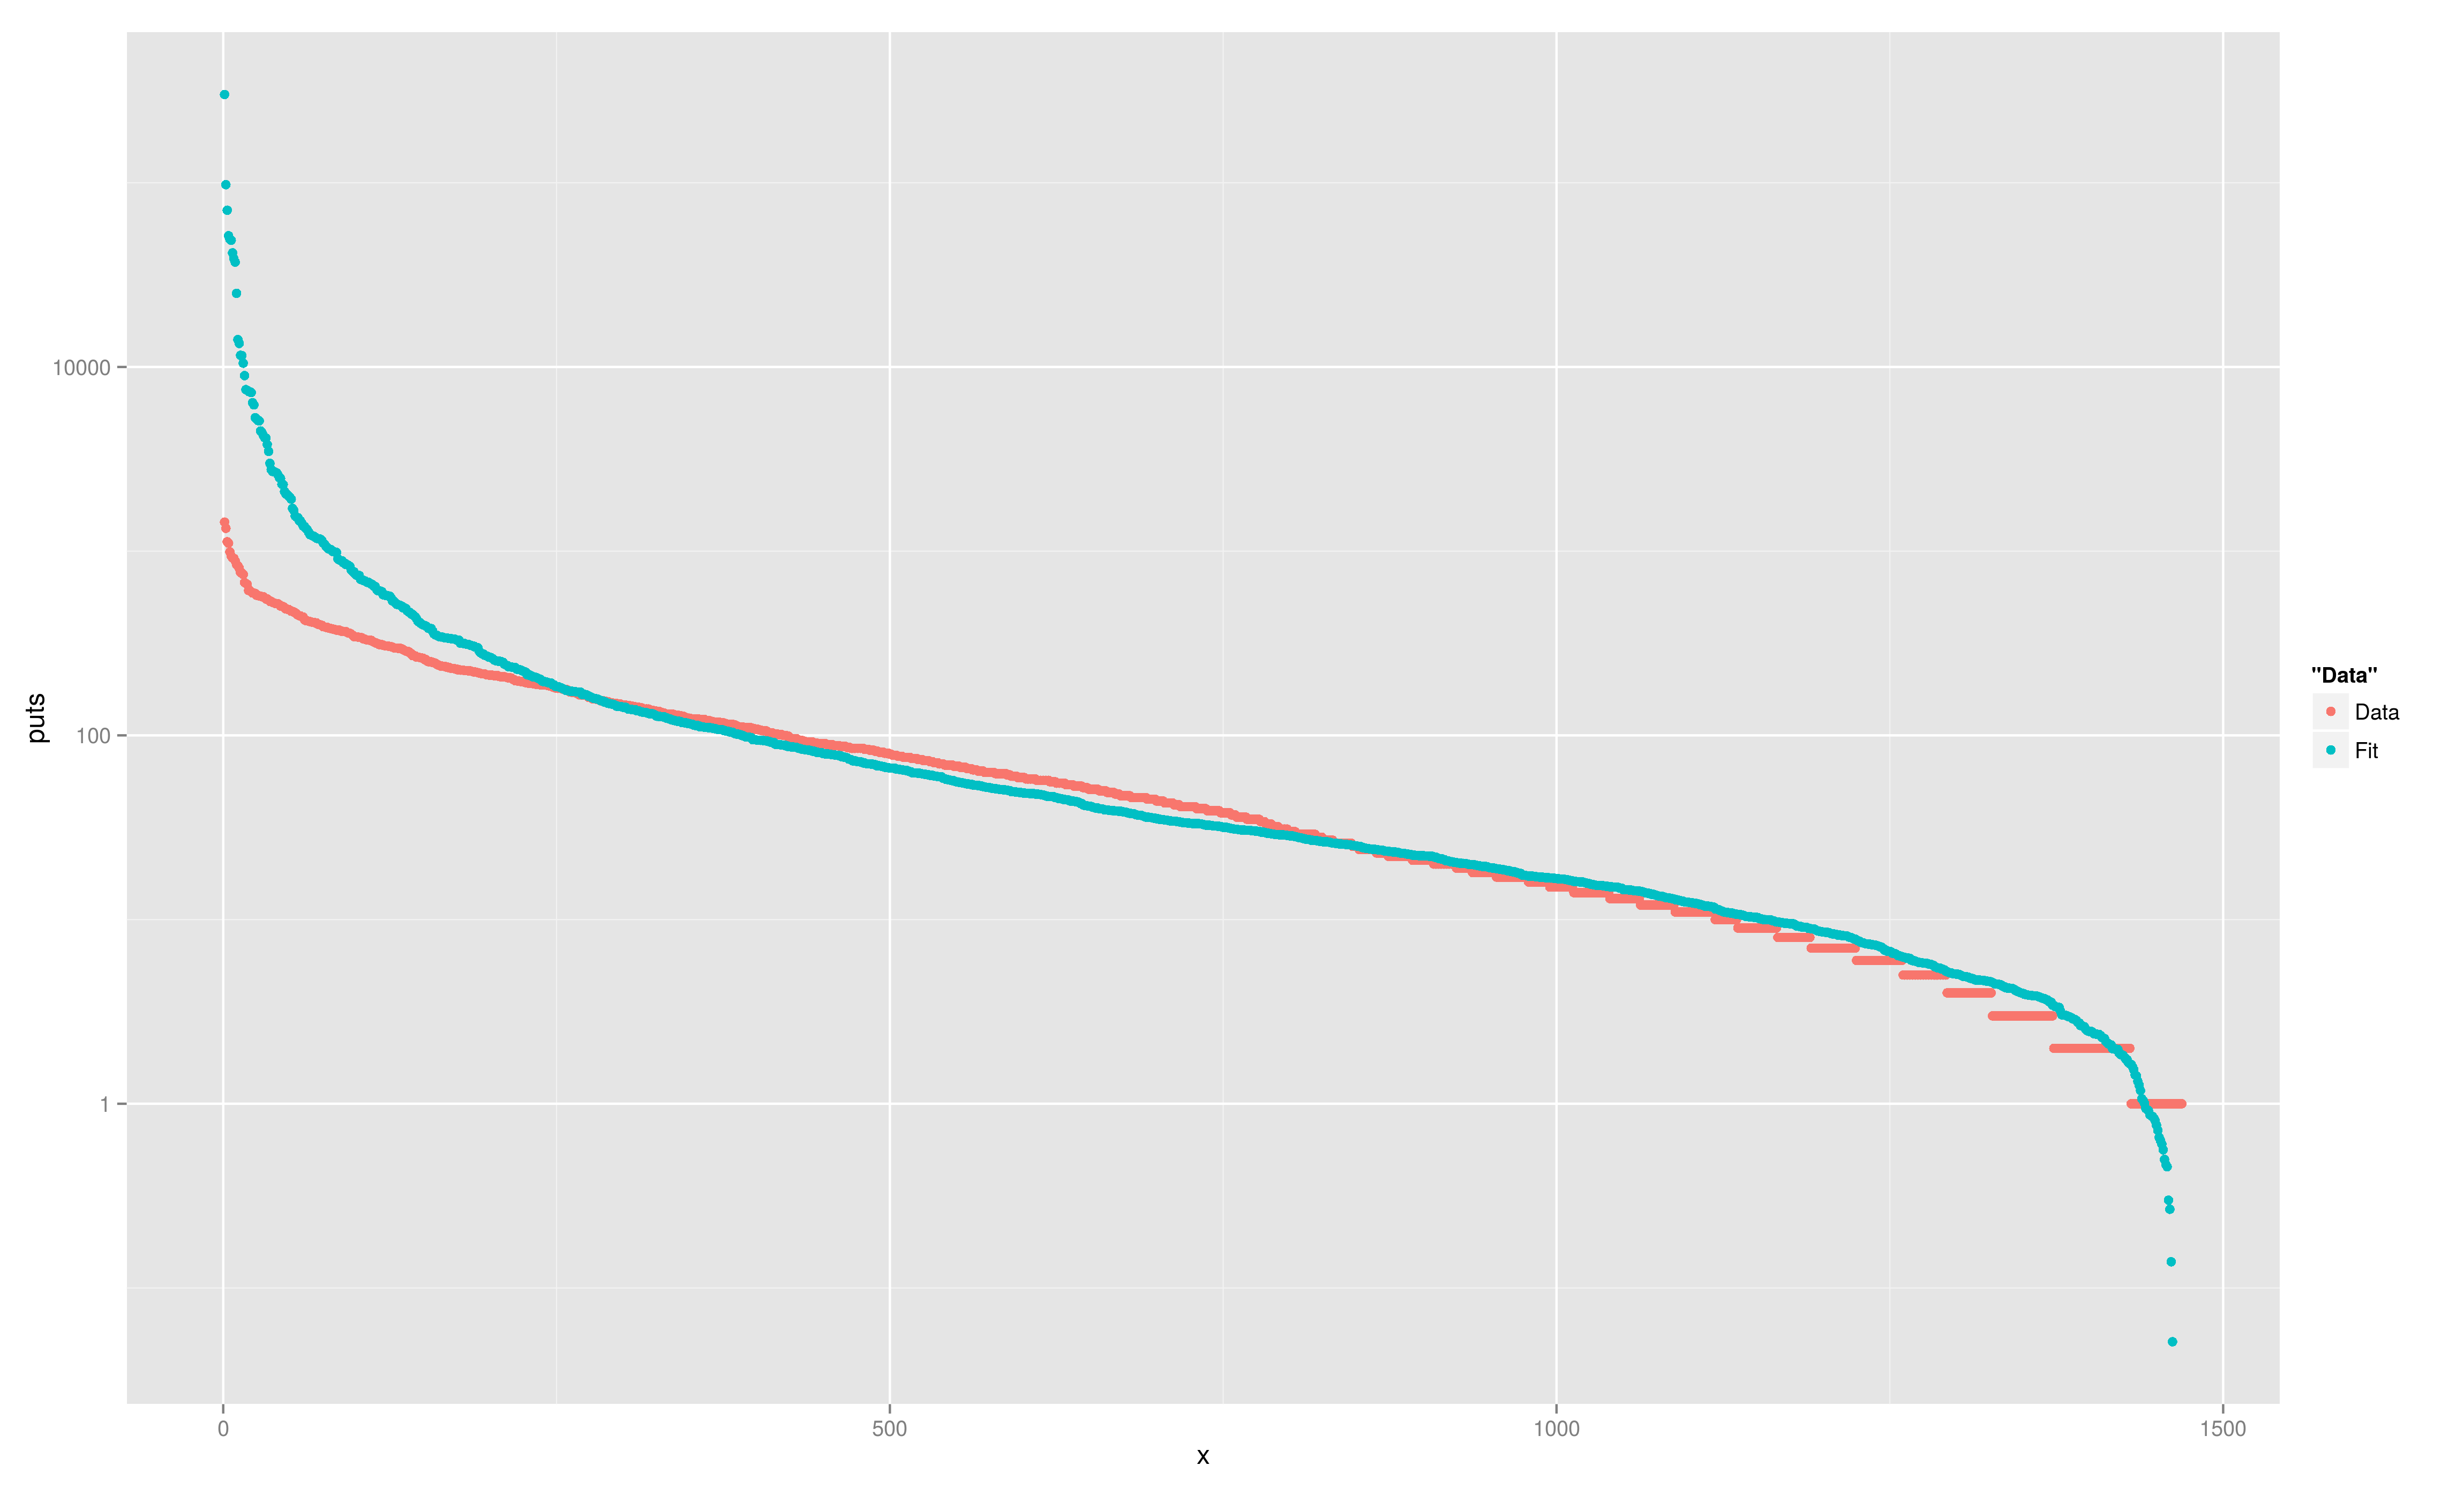
\includegraphics[width=0.49\linewidth]{img/gev-fit-ww.png}
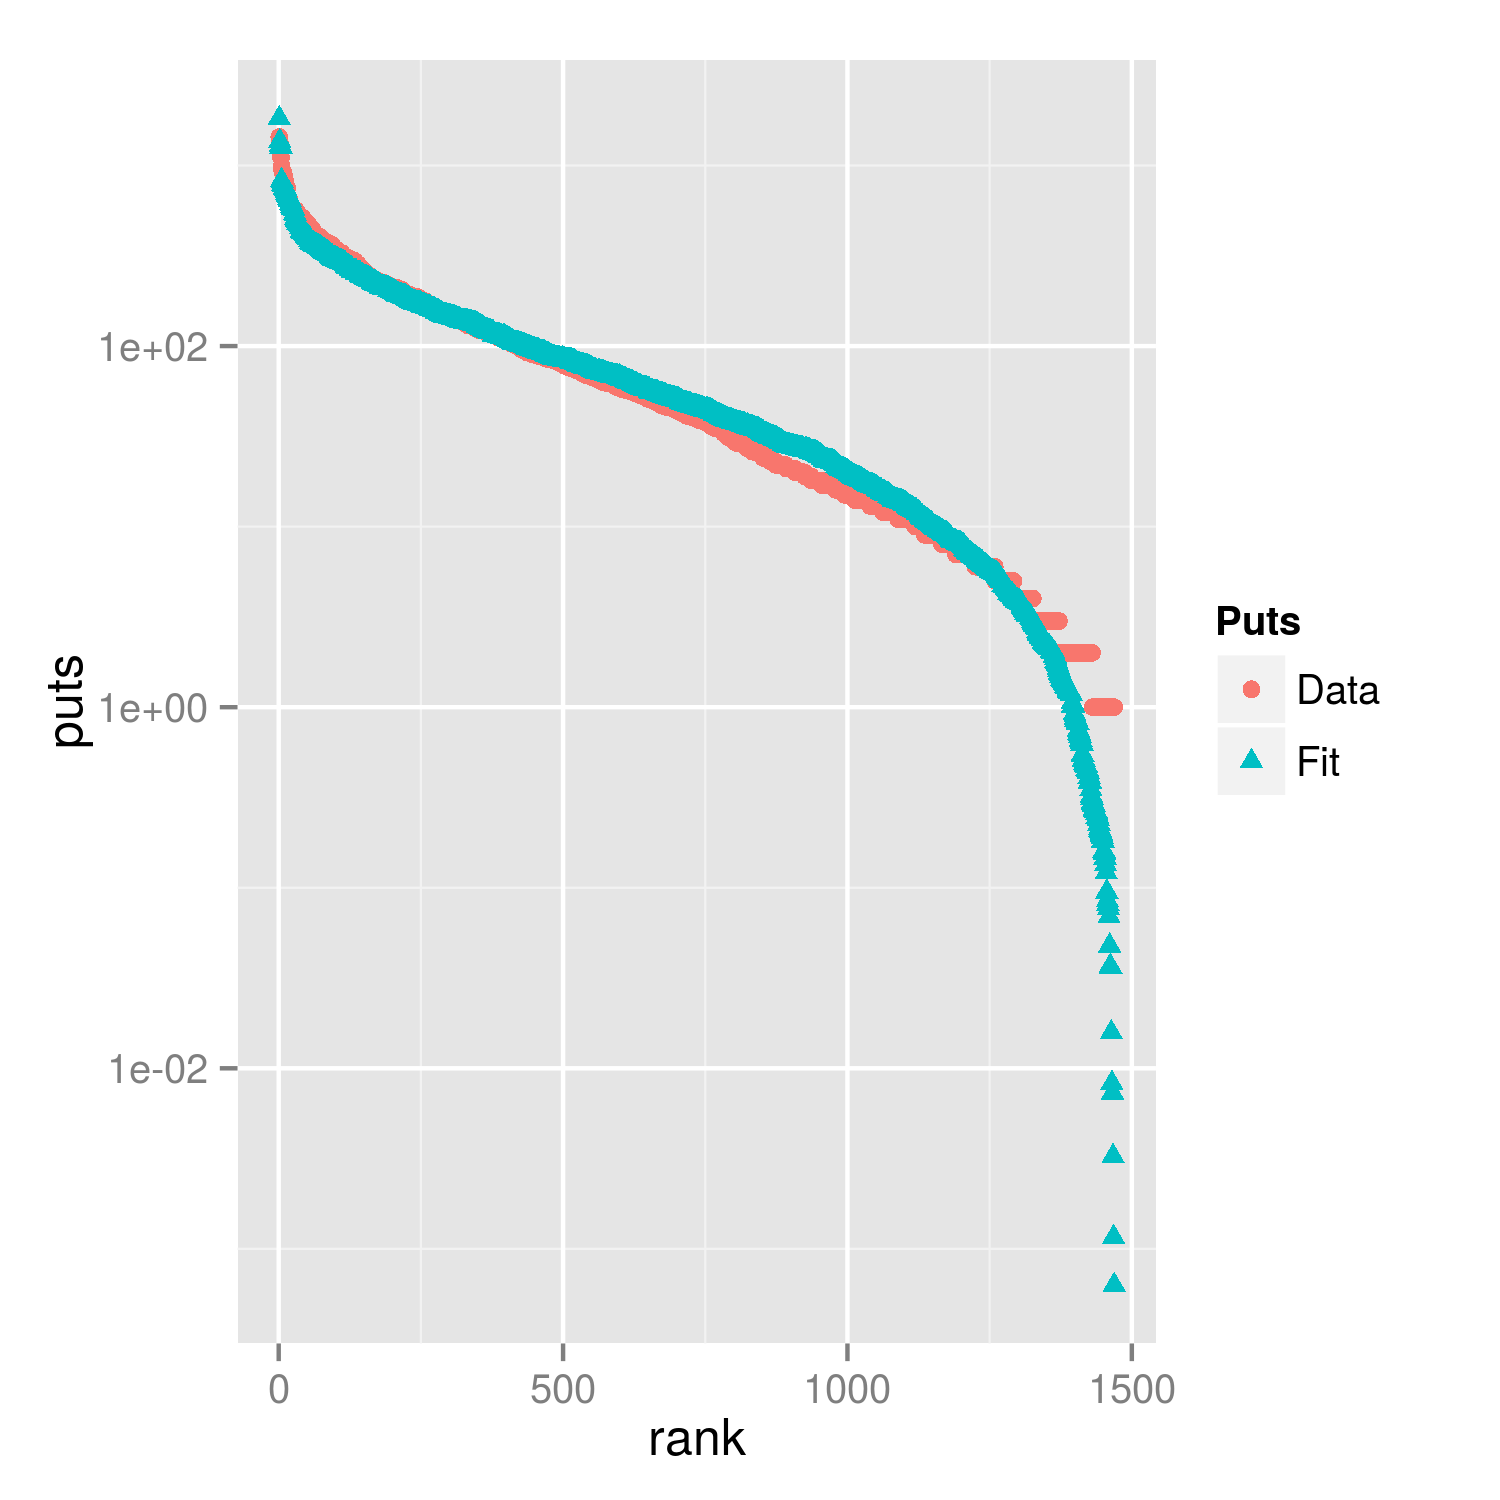
\includegraphics[width=0.49\linewidth]{img/weibull-fit-ww.png}
\caption{Ranked number of {\tt PUT}s per worker and GEV fit (in red, right) and Weibull (in red, left) for the {\sf NodIO$^2$} model. }  
\label{fig:gev:w2}
\end{figure}
%
It is also interesting to measure the scaling properties in this
model, that is, the relationship between the number of IPs
participating in an experiment and the time it takes to complete
it. This is shown in Figure \ref{fig:ipstime:w2}, which shows every
experiment in a time (in milliseconds) vs. number of workers participating
in it. Although there is not a clear trend, the graph seems to say
that the time needed for finding the solution in this evolutionary
algorithm does not depend on the number of workers participating in
it. This does not mean that it is independent on the number of {\em
  simultaneous} users, which is probably the case although it is more
difficult to measure. There seems to be a trend towards a decreasing
standard deviation in the time, with more volunteers adding {\em
  robustness} to an experiment and certainty in the time it is taking;
however, more experiments would be needed to check this hypothesis.

As we did in the previous subsection, we have fitted also the number
of HTTP {\tt PUT}s per worker to a  Generalized Extreme Value (GEV) function, with the result shown %FERGU: he cambiado GEV por GET (lo de GEV era un error, no? vayamos a que sea algo nuevo que no conozco...)
%cojollos, Fergu, si no conoces no lo cambies. 
in Table \ref{tab:puts:ww}. Comparing this table with what we obtained
in the previous experiment, Table \ref{tab:puts:os}, we find higher values
for the location $\mu$ and scale $\sigma$ parameters, accounting for
the higher number of contributions per volunteer that has been
previously observed; however, the shape $\xi$ parameter is
substantially similar, with a {\em bell} shape leaning towards the
origin, indicating a pattern of a few users with many contributions
and many with few contributions. If we plot the model and the data
side by side, as shown in Figure \ref{fig:gev:w2} we see that the fit
is not so tight as in the previous case, with the model overestimating
the number of individuals with a high number contributions. This is
probably due to the fact that in the previous case, the user needed to
voluntarily reload the page to contribute the most generations, with a
{\em phase change} between the people that did so and the people that
just run the experiment until completion. In this case, however, the
user just needs to let it run, without that phase change and thus a
more {\em equalitarian} distribution of contributions, which rather
corresponds to a Weibull function, as shown in Figure
\ref{fig:ipstime:w2} (right hand side). The fitted parameters for this
distribution, shown in Table \ref{tab:puts:ww}, show a shape parameter
equal to 0.69, a value that is remarkably similar to the 0.5 value
found for time devoted to games in Chambers et
al. \cite{chambers2005measurement}.

In general, this second version of the {\sf NodIO} framework and the
single experiment performed prove that it can be the foundation for a
high-server-performance distributed evolutionary computation platform,
providing reasonable algorithmic performance and being, in general,
easy to use with a straightforward modification of the fitness
function. 

%---------------------------------------------------------------
\section{Conclusion}
\label{sec:conclusion}

In this paper a client-server architecture for volunteer and distributed
evolutionary algorithms that uses the browser, termed {\sf NodIO} and
based on the {\sf NodEO} evolutionary algorithm library has been evaluated. 

In order to establish a baseline performance, the evolutionary
algorithm was run in a desktop client-program written in JavaScript
using NodEO to solve the 40-trap function. The first experiments with
{\sf NodIO} proved that, although obtaining better performance than de
baseline was possible, it did not happen, mainly because of the
difficulty in carrying over volunteers to other experiments when the
one they were participating on was finished, shown in the low
correlation between the number of IPs in successive experiments. This
also resulted in a low number of generations allotted by users. 

In the second implementation, {\sf NodIO$^2$}, Web Workers
were used so that several clients per browser could be executed and
they could run in the background, so that the the number of
generations per user could be improved. The number of generations per
user increased to the point that baseline performance was overcome in
most cases. The architectural changes led to a high correlation
between successive experiments, so that, even as the median number of
volunteers per experiment decreased, they were probably contributing
to the experiment at the same time, so that our objective was
achieved. In general, one of the first conclusion for this paper is
that the browser technologies should be used to its full extent so
that the user time is leveraged to its full potential, and this was
achieved with {\sf NodIO$^2$}.

%---------------------------------------------------------------
% use section* for acknowledgment
\section*{Acknowledgment}

This work has been supported in part by TIN2011-28627-C04-02 and.
TIN2014-56494-C4-3-P (Spanish Ministry of Economy and Competitivity),
SPIP2014-01437 (Direcci{\'o}n General de Tr{\'a}fico) and PYR-2014-17
GENIL project (CEI-BIOTIC Granada). We would also like to thank the
anonymous reviewers of previous versions of this paper who have really helped us to improve
this paper (and our work) with their suggestions. We are also grateful
to Anna S\'aez de Tejada for her help with the data processing scripts.


\bibliographystyle{IEEEtran}
\bibliography{geneura,volunteer,javascript,ror-js,GA-general}

\end{document}
%%% Local Variables:
%%% ispell-local-dictionary: "english"
%%% End:
